\documentclass{article}
\usepackage{iclr2024_conference_mod,times}
\preprintcopy
\usepackage{amsmath,amssymb,amsthm}
\usepackage[T1]{fontenc}
\usepackage[utf8]{inputenc}
\usepackage[hidelinks]{hyperref}
\usepackage{url,xurl}
\usepackage{graphicx,booktabs,float,multirow,tabularx,xltabular}
\newcolumntype{Y}{>{\raggedright\arraybackslash}X}
\usepackage{inconsolata}
\usepackage{enumitem}
\usepackage{microtype}
\usepackage[capitalize]{cleveref}
\usepackage[compact]{titlesec}
\usepackage{caption,subcaption}
\usepackage{xcolor}
\newtheorem{proposition}{Proposition}
\newtheorem{corollary}{Corollary}
\setlength{\emergencystretch}{3em}
\newcommand{\nats}{\,\mathrm{nats}}
\newcommand{\ci}[2]{[#1,\,#2]}
\newcommand{\head}[2]{L#1h#2}
\newcommand{\fig}[1]{\IfFileExists{#1}{\includegraphics[width=\linewidth]{#1}}{\fbox{\parbox[c][1.6in][c]{0.96\linewidth}{\centering\path{#1} (pending)}}}}

\title{A Circuit for In-Context Learning}
\author{Andrew Gao\thanks{Correspondence to gaodrew@stanford.edu. Code and batteries: \url{https://github.com/andrewgcodes/in-context-learning-circuit}.} \\
Stanford University
\And
William Gao \\
Stanford University}

\begin{document}
\maketitle
\vspace{-7mm}\noindent\begin{minipage}{\linewidth}\centering
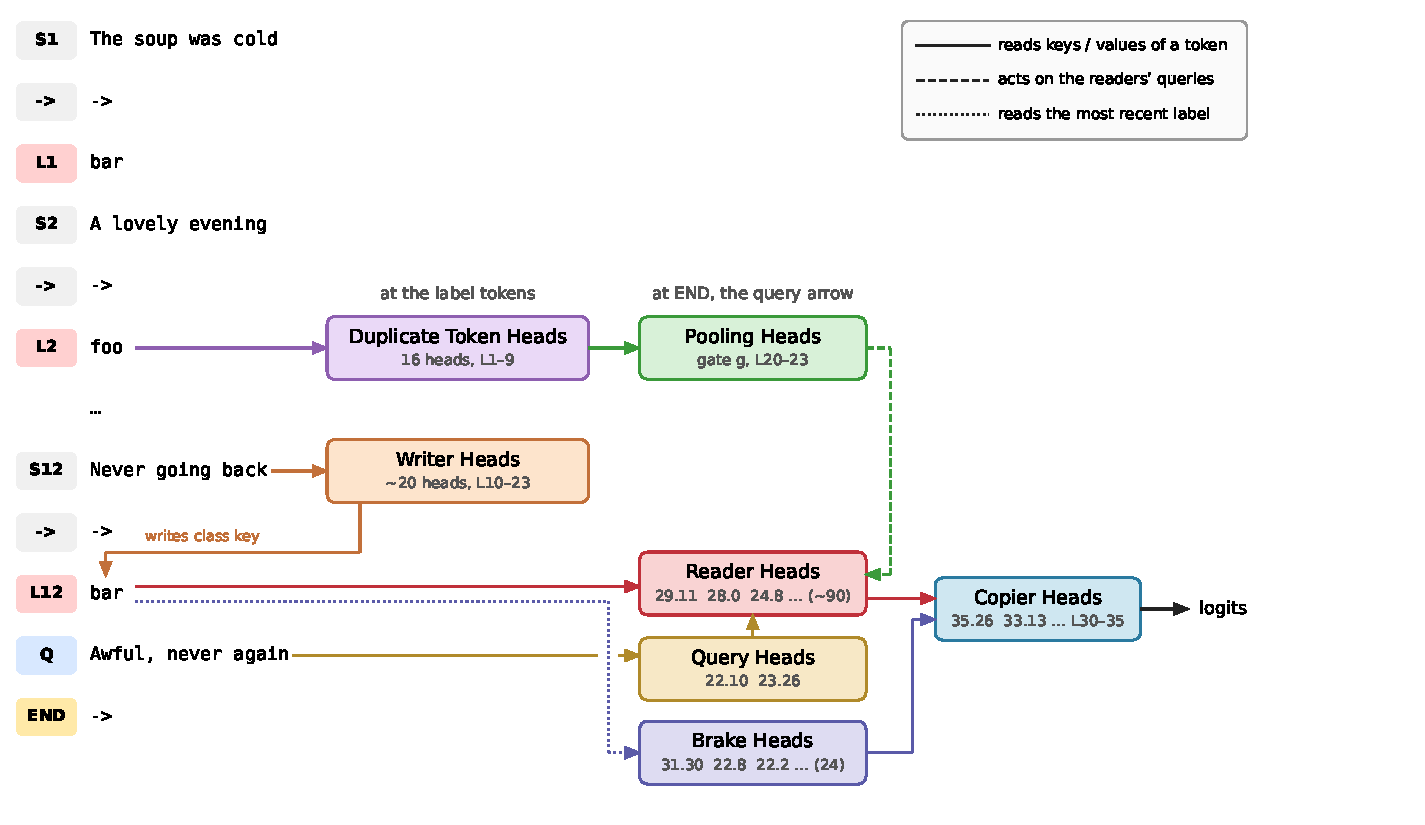
\includegraphics[width=0.78\linewidth]{figures/fig1_circuit.pdf}
\end{minipage}\vspace{-3mm}

\begin{abstract}
In-context learning (ICL), a pretrained language model's ability to perform a task specified by demonstrations in its prompt, needs no training objective and no parameter updates. With arbitrary labels the model must acquire a mapping it cannot have memorized, so the learning happens within a single forward pass. Prior work found candidate parts but not how they compose. We give the composition for few-shot sentence classification with arbitrary labels in three 3--4B-parameter transformers. The model implements a key-value memory over label-token positions: each label token's residual stream encodes the label's identity, and middle-layer attention heads write into it the class of the preceding demonstration as its key. At the query, upper-layer heads match the query's class against the stored keys and copy out the matching labels. An early-layer signal encoding whether any label has repeated gates this readout; in its absence the readers attend to the beginning of the prompt and no label is favored, a default that softmax normalization makes unavoidable. A separate set of heads suppresses the most recently seen label, removing a recency bias. Each step is established causally by activation patching between minimal-pair prompts, head ablations against random-head baselines, and steering with the model's own signals. Cutting the connections shows that sixty percent of a class flip passes through the readers and that a few amplified readers cannot replace the rest. A three-constant softmax model of the readout, fit on one prompt distribution, predicts another. The computation is conserved across the three models; which heads fill each role varies. The named heads alone reproduce the behaviour, and a transformer trained from scratch grows the same parts, the gate only when retrieval is penalised. The circuit transfers to semantic concepts; with the concept's own words as labels, the same reader and brake types carry the part of the margin that follows the demonstrations, while the part that follows word meaning lies outside it. The same parts, with a causal gate, appear from 0.6B to 8B in one family; across that range the brakes' hold on word meaning rises with the flipped-label margin, the behaviour \citet{wei2023larger} found only in large models, and the base model's heads still carry retrieval after instruction tuning. ICL in this setting is a gated associative lookup built from a few identifiable component types, traced causally from demonstrations to prediction.
\end{abstract}
\section{Introduction}\label{sec:intro}
Show a base language model a dozen lines like these,
\begin{quote}\small\ttfamily
The soup was cold and the waiter rude -> bar\\
A gorgeous evening with old friends -> foo\\
\ldots\\
I would not go back to that place ->
\end{quote}
and it answers \texttt{bar}. Nothing in pretraining taught it that \texttt{foo} means a pleasant evening or that \texttt{bar} means a bad meal. The model worked that out from the prompt, in a single forward pass, with no change to its weights. This is few-shot in-context learning~\citep{brown2020fewshot}. It is one of the abilities that turned language models into general tools, and labeling sentences is its simplest form. That simplest form is what we study. Instructions, long-form tasks and many-class binding are outside the scope of this paper.

Several pieces of the answer are known. Induction heads copy a token that followed an earlier copy of the current token~\citep{olsson2022induction}. Task vectors and function vectors~\citep{hendel2023taskvectors,todd2023fv} show that a handful of heads carry a compact description of the demonstrated task at the query. Label tokens are where task information accumulates~\citep{cho2024circuit,zheng2024labelwords,hu2025addition}, and the recency bias of in-context learning has been traced to query--key similarity with label positions~\citep{yu2024qk}. Nobody has joined these pieces into one working algorithm. We do not know, precisely, what is written at the label tokens and on which side of attention. We do not know what reads it, or how that read is switched on and off, or how the result travels to the logits. And we do not know which of the parts are single heads one can name and which are populations that only act in sum.

This paper gives that account for two-class label retrieval and function selection on invented-word and natural labels, at up to twelve demonstrations, in three base models of three to four billion parameters (Qwen3-4B, SmolLM3-3B, Llama-3.2-3B). In the field's terms, we describe a circuit and the algorithm it implements; Figure~\ref{fig:algorithm} draws it as a circuit, Figure~\ref{fig:lanes} lays it along the layers, and Figure~\ref{fig:walkthrough} places it on one prompt. The demonstrations become a key--value memory in the prompt. Each label token becomes a slot. Its value is the label's own identity. Its key is the class of the sentence it followed, deposited into the label token by about twenty mid-layer heads that read the sentence and write into the label (K-composition in the sense of \citealt{elhage2021framework}). At the query the model computes the new sentence's class. About ninety heads in the upper layers then compare that class with the slot keys through an ordinary softmax over positions and copy the values of the slots that match; they behave as class-keyed induction heads. The read is gated. A direction in the residual stream, computed by early duplicate-token heads from whether any label has appeared twice, lowers the logit those readers assign to the attention sink at position zero. When no label repeats the sink wins and the model emits nothing in particular. We call this the null action, and it follows from the softmax: mass must go somewhere, and the sink is the only position that carries no prompt. A further population of about two dozen heads writes against whichever label the model has just seen. These are negative heads in the sense of \citet{wang2022ioi} and \citet{mcdougall2023copysuppression}. We call them brakes, because removing them triples the margin and makes the model recency-biased.

Every step rests on an intervention with a matched control. We swap one sentence, one label, or one query between twin prompts that are token-identical elsewhere, and hand the resulting activations into the intact run head by head, group by group, or position by position. We knock heads out against random heads of the same number and layers. We push directions into the residual stream at the dose the model itself uses, against random directions of the same norm. Every head set chosen on one draw of prompts is confirmed on a fresh draw. Where the model concentrates a function in a few heads we name them. Where it spreads a function over many, we characterize the population by the direction it reads or writes and show that the direction is specific against a random subspace of the same dimension. The answer is also accounted for exactly: on each prompt, the contributions of every head and MLP to the answer logit sum to the logit the model produces, to within 0.05 nats.

Two things surprised us. The read obeys a simple law. Each reader's mass on the matching slots follows a three-constant softmax expression in the number of matching slots, the number of slots and the null logit. The constants fitted on twelve-demonstration prompts predict a one-slot-per-class regime that was never fitted, in Qwen and in Llama. The same constants fail on longer prompts. That failure says a head's null mass and its total matching mass are constants of the head, so adding matching slots divides a fixed budget among them. The second surprise is that half of the links are populations for a reason we can state. A single reader already separates the two classes in its attention pattern. What no head has is the output gain to write the answer alone; no head writes more than 0.2 nats of logit, and a 1.3-nat answer therefore needs at least seven.

Section~\ref{sec:setup} describes the prompts, measures and interventions. Sections~\ref{sec:slot}--\ref{sec:accounting} follow the computation from the slot, through the read, the gate and the query code, to the readers, brakes and the final logits. Section~\ref{sec:replication} asks which parts of the account must hold in any transformer and which are choices made by training, and tests the account in two further models and across training checkpoints. Section~\ref{sec:discussion} states what the account does not cover, including two predictions that did not hold.

\begin{figure}[t]\centering
\fig{figures/fig8_walkthrough.pdf}
\caption{One twelve-demonstration prompt, stage by stage. Columns are tokens (sentences $s_i$, arrows, labels, the query $q$); rows are layers of Qwen3-4B. Each coloured block marks the tokens and layers at which a stage acts: duplicate detectors and the encoder early, writers into the label tokens in the middle layers, then at the query arrow the query code, the gate, the readers, the brakes and the readout band. Later sections give the intervention behind each block.}
\label{fig:walkthrough}
\end{figure}

\section{Setup}\label{sec:setup}
\paragraph{Prompts.} Every prompt in the paper is a list of demonstrations, one per line, written \texttt{sentence -> label}, followed by a query sentence and an arrow. The model's next token is the answer. We use four batteries. The \emph{concept} battery has six demonstrations, three per class, on sentence axes such as topic (animals against food), sentiment, language (English against Spanish) and question against statement, with invented-word labels (\texttt{foo}/\texttt{bar}, \texttt{quil}/\texttt{zorp}) and natural ones. The \emph{concept12} battery has twelve demonstrations, six per class. The \emph{slotgate} battery has four demonstrations and comes in token-identical pairs: in one member each label appears twice, in the other every label appears once, so the pair differs only in whether labels repeat. The \emph{manyclass} battery has two to six classes with one or more demonstrations each and arbitrary single-token labels. Appendix~\ref{app:prompts} shows one verbatim prompt from each. All labels except \texttt{zorp} are single tokens in all three tokenizers; for a two-token label, the first token carries the key.

\paragraph{What we measure.} The margin of a prompt is the log-probability of the correct label minus that of the other label, scored over the full token sequence of each. A positive margin means the model prefers the right answer; a margin of 2 nats means it prefers it by a factor of about seven. The effect of an intervention is the change in margin it causes, paired prompt by prompt against the intact run, and every effect is reported with a 95\% interval from a paired bootstrap over prompts (4000 resamples). When we say a head set ``costs $-0.74$ nats'', we mean knocking it out lowers the margin by that much on average.

\paragraph{Twins.} Most interventions use twin prompts: two prompts that are identical token for token except inside one span. We use five twins. The class-flipped sentence replaces one demonstration's sentence by one of the other class. The same-class sentence of equal length is the same-answer control. The label exchange swaps \texttt{foo} and \texttt{bar} everywhere. The other-class query replaces the query sentence. The unique-label rewrite replaces each repeated label by a fresh one. Because the twins are aligned token for token, we can take any activation from one and place it into the other at the same position, and ask how much of the twin's effect that activation carries. We call this a handoff.

\paragraph{Interventions.} A \emph{knock} mean-ablates a head's output over the battery, which removes what the head writes without zeroing it. A \emph{handoff} replaces a head's, group's or layer band's queries, keys, values or output at chosen positions with the twin's. A \emph{push} adds a direction to the residual stream at the query arrow at the dose the model itself uses (the difference in projection between twins), with a random direction of the same norm as control. A \emph{hold} fixes a downstream component at its intact value while an upstream handoff runs, which tells us whether the upstream effect passes through that component. All of these are forward hooks on the HuggingFace implementations in bfloat16 on one H100. Alongside them run the loupes: per-head attention rows at chosen layers, per-head and per-MLP direct contributions to the answer logit, and projections of the residual stream on fitted directions.

\paragraph{Controls.} Every named head set is compared with random sets of the same size drawn from the same layers. Every direction push is compared with a random direction of the same norm. Every set selected on one draw of prompts is confirmed on a fresh draw from the same pools with a different seed, and the numbers we lead with are from the fresh draw.

\paragraph{Models.} Qwen3-4B-Base (36 layers, 32 query heads, 8 key--value groups, QK-norm), SmolLM3-3B-Base (36 layers, 16 heads, 4 groups) and Llama-3.2-3B (28 layers, 24 heads, 8 groups), plus intermediate checkpoints of OLMo-2 1B and 7B for the emergence study. We write L$\ell$h$h$ for head $h$ of layer $\ell$, zero-indexed.

\section{Where is the memory? (the slot)}\label{sec:slot}
\begin{figure}[t]\centering
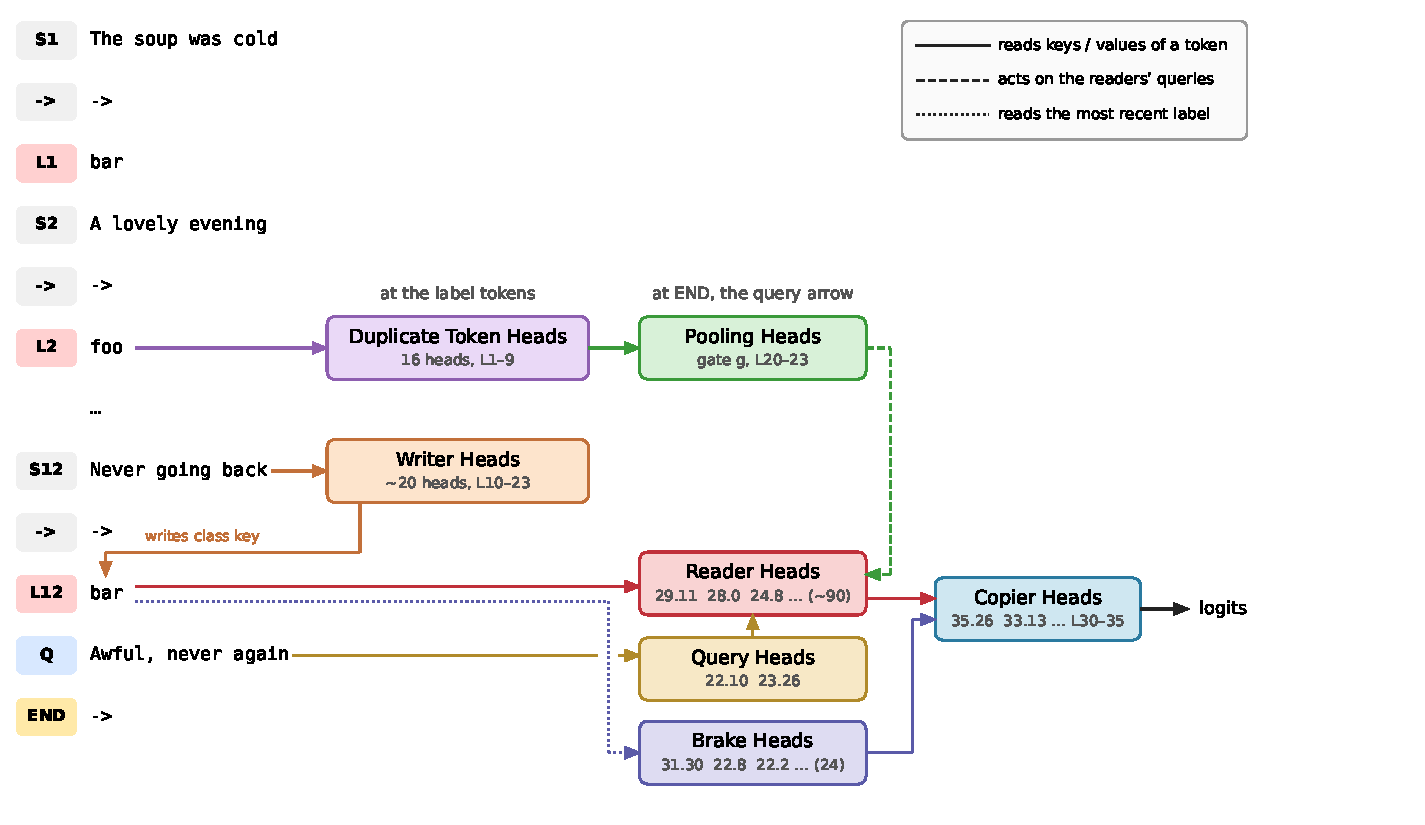
\includegraphics[width=\linewidth]{figures/fig1_circuit.pdf}
\caption{The circuit for few-shot in-context learning in Qwen3-4B-Base. Prompt tokens run down the left (sentences $S_i$, labels $L_i$, the query $Q$ and its arrow END); boxes are classes of attention heads with layer.head beneath. Writer Heads give each label token a key (the class of its sentence) next to its value (the label); at END, Reader Heads match the query's class against those keys and copy the matching labels, Copier Heads write the logits, Brake Heads write against the most recent label, and the gate $g$ (Pooling Heads) opens the read by lowering the readers' attention-sink logit (dashed). Section~\ref{sec:slot} onward gives the intervention behind each arrow.}
\label{fig:algorithm}
\end{figure}

\begin{figure}[t]\centering
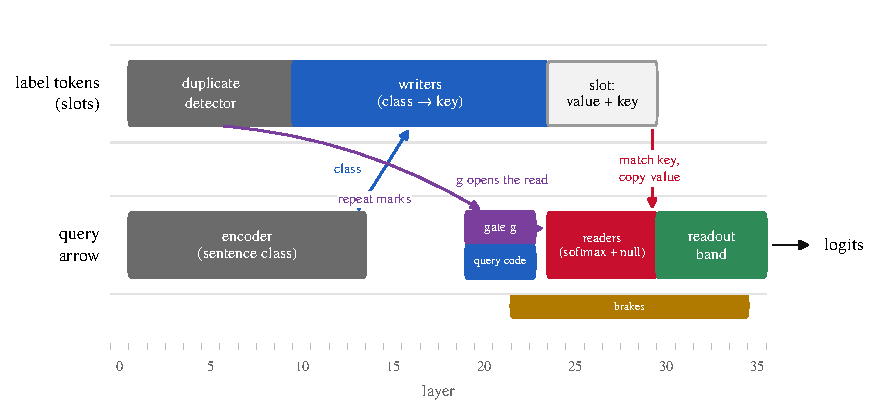
\includegraphics[width=\linewidth]{figures/fig1_algorithm.pdf}
\caption{The same circuit laid along the layers of Qwen3-4B-Base. Top lane: what happens at the label tokens (duplicate-token heads mark a repeated label; writers deposit the sentence's class into the label's residual stream, making it a slot with a value and a key). Bottom lane: what happens at the query arrow (the encoder computes the query's class; the pooled repeat signal $g$ lowers the readers' sink logit; readers match the query class against the slot keys and copy the matching values; the readout band and late MLPs write the logits, with the brakes writing against the last label).}
\label{fig:lanes}
\end{figure}

\begin{figure}[t]\centering
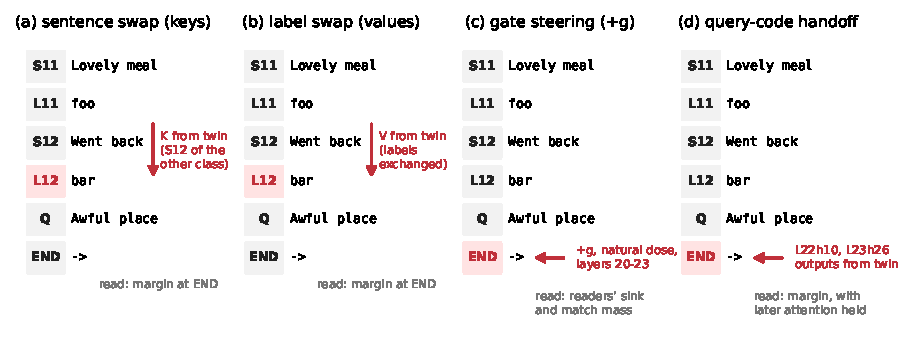
\includegraphics[width=\linewidth]{figures/fig18_interventions.pdf}
\caption{The four interventions. Each panel shows the end of a 12-shot prompt; the red component is replaced or steered and the output is read at END. (a)~Sentence swap: the keys at the label token are taken from the twin prompt whose demonstration sentence belongs to the other class, so the slot's key no longer matches its value. (b)~Label swap: the values at the label token are taken from the twin with the labels exchanged. (c)~Gate steering: the model's own gate direction $g$ is added at END at its natural magnitude before the reader layers, and the readers' attention to the sink and to matching slots is measured. (d)~Query-code handoff: the outputs of the two query heads at END are taken from the twin with the query of the other class; later attention outputs can be held fixed to test whether the effect passes through them.}
\label{fig:interventions}
\end{figure}

\begin{figure}[t]\centering
\fig{figures/fig15_slot.pdf}
\caption{Anatomy of a slot. The residual stream at a label token holds two things read through two different matrices. The label's identity arrives from the token's own embedding and early layers and is read by the readers' $W_V$; the class of the sentence it followed is written in by middle-layer heads that attend back to the sentence, and is read by the readers' $W_K$ as the key the query class is matched against.}
\label{fig:slotanatomy}
\end{figure}

After the model has read twelve demonstrations, where is the information it will need? Each demonstration has a sentence and a label, and the model will later need to know, for each demonstration, which class the sentence belonged to and which label followed it. Both pieces end up in the same place: the residual stream of the label token. We call that residual a slot, because it behaves like one cell of a key--value memory. Its value is the label's own identity. Its key is the class of the sentence that came before it. The two live on different sides of attention, and two experiments pull them apart.

The first experiment exchanges the labels. Take a prompt and swap \texttt{foo} and \texttt{bar} throughout, leaving every sentence where it is. The right answer to the query is now the other label, and the model's margin flips sign. To find which activations carry the flip, we hand the swapped prompt's keys and values at the label tokens into the intact run. Handing them at every layer reproduces the flip exactly ($-7.18$ nats in Qwen, $-5.55$ in SmolLM3, $-4.92$ in Llama), but that is a check of the harness, not a finding: two prompts that differ only at the label tokens have identical inputs everywhere else, so replacing the label tokens' keys and values at every layer makes every other position compute exactly what it computes in the swapped prompt, in any transformer, by induction over layers (Appendix~\ref{app:induction}). The informative handoffs are the restricted ones. In SmolLM3, keys and values at the label tokens in the reader layers 21--29 alone carry $-2.94$ of the $-5.55$. In Qwen the values of the 72 layer-21--29 key-value groups at the label tokens carry 86\% of the exchange, and the eight sharpest readers' values $-2.16$; the keys alone carry $+0.56$, nothing. So the label's identity sits in the value side of the slot, and it is read in the upper layers. It is not spread evenly over the value side: handing the values of single key-value groups shows three of the 72 groups in layers 21--29 carrying about half of the exchange's effect, and one group in layer 24 a quarter (Figure~\ref{fig:transport}).

The second experiment leaves the labels alone and changes a sentence. Replace one demonstration's sentence by a sentence of the other class, so that \texttt{foo} now follows a complaint instead of a compliment. This also moves the answer, by $-2.87$ nats on the six-demonstration battery. Now the effect runs through the keys. Handing the changed prompt's keys at the label tokens in layers 21--29 carries $-2.35$ of it; the eight sharpest readers' keys carry $-0.55$ and their values $+0.10$. In Llama the same experiment localizes the key to the label tokens' K/V in the middle layers only: layers 7--13 and 14--20 each carry $-0.15$ of a $-0.23$ twin effect, while layers 0--6 and 21--27 carry $-0.02$ and $-0.04$. Early layers have not written the key yet, and late layers have already read it. Figure~\ref{fig:writers}a shows the profile.

A control tells us the second experiment measures the class and not the sentence. Replacing a demonstration's sentence by a different sentence of the same class and the same token length moves the answer by $+0.08$ nats, with every handoff from that twin inside $\pm0.06$. Whatever the slot stores about its sentence, only the class part reaches the answer.

How does the class get into the label token? The label token does not see its sentence directly; attention must carry it. About twenty heads in layers 10--23 do so. Each attends from the label token back to the words of its own sentence and writes the class direction into the label's residual. No one of them carries more than 5\% of the effect and the top twenty together carry 64--92\%; knocking six named writers does no more than knocking six random heads of the same layers. The class they write is one direction $u$ per task, the same for both labels (held-out sign agreement 0.95--1.00), so a two-class key needs one dimension. Writing it must be spread across depth. Adding the same total dose of $u$ to the label tokens in one layer helps less than spreading it over four layers. In SmolLM3, on the 144 prompts of the axes the model does not bind on its own (with the query's class pushed as well), the single-layer write at layer 16 gains $+0.37$ \ci{+0.29}{+0.46} and the same dose spread over layers 12, 14, 16 and 18 gains $+0.56$ \ci{+0.48}{+0.65}. At double dose the single-layer write falls back to $+0.20$ \ci{+0.09}{+0.31} where the spread write keeps climbing ($+0.69$ \ci{+0.58}{+0.81}; Figure~\ref{fig:writers}b). We read this as the writers being contextualisation heads: each layer's write is read and reshaped by the next, and a dose dumped in one place does not get the same treatment.

The slot is also the bottleneck. Features the model never represents linearly at the arrow (word parity, the third letter, digit rules) never bind at any number of demonstrations. Writing $u$ into the slots of such a prompt by hand lifts accuracy from 50 to 71\%; key-only, query-only and random directions stay within $\pm0.1$ (Appendix~\ref{app:encoder}). If the key is there, the rest of the circuit works; if it is not, no amount of reading helps. The next question is how the reading works.

\begin{figure}[t]\centering
\fig{figures/fig2_slot.pdf}
\caption{The slot holds a value and a key on different sides of attention. (a) Exchanging the labels: the effect runs through the label tokens' values in all three models. (b) Changing a sentence with the label fixed: the effect runs through the label tokens' keys, in the middle layers only. (c) A same-class sentence of the same length moves the answer by at most 0.06 nats. Bars are paired effects on the margin with 95\% bootstrap intervals; grey bars are size-matched random controls.}
\label{fig:slot}
\end{figure}

\begin{figure}[t]\centering
\fig{figures/fig13_transport.pdf}
\caption{Three KV groups carry half of the label's value. Handing the values of all 72 layer 21--29 KV groups at the label tokens, from a prompt with the labels exchanged, carries 86\% of the exchange's effect on the margin (left). By layer, the effect sits in layers 22, 24 and 29 (right, grey); within each, one KV group carries most of it (red): group 24.5 alone carries a quarter, groups 24.5, 29.2 and 22.5 together about half. Random head sets of the same size move the margin by 0.03 or less (dotted). Qwen3-4B, 12-shot invented-label prompts, 72 prompts.}
\label{fig:transport}
\end{figure}

\begin{figure}[t]\centering
\fig{figures/fig14_writers.pdf}
\caption{The key is written in the middle layers, and the write must be spread. (a) In Llama-3.2-3B, handing the sentence-exchanged prompt's label-token keys and values per layer band: the two middle bands carry the effect, the first and last almost none. (b) In SmolLM3, adding the same total dose of the class direction $u$ to the label tokens in one layer helps less than spreading it over four, and falls back at double dose where the spread write keeps climbing (95\% intervals; 144 prompts).}
\label{fig:writers}
\end{figure}

\section{What reads it? (Reader Heads and the read law)}\label{sec:read}
With the memory in place, the query has to be looked up in it. The lookup is done by attention heads. Each reader performs an ordinary softmax over the prompt's positions. The attention sink at position zero takes part in that softmax as a position with no content. The mass a reader puts on the right slots follows a three-constant expression that we can fit in one regime and test in another.

\paragraph{Notation.} Write $h_q$ for the residual stream at the query arrow when a reader head runs, and $r_j$ for the residual at the $j$-th label token. The head forms $q = \mathrm{RoPE}(\gamma_q \odot \mathrm{norm}(W_Q h_q))$ and $k_j = \mathrm{RoPE}(\gamma_k \odot \mathrm{norm}(W_K r_j))$, where norm is the per-head RMS normalization Qwen applies and $\gamma$ its gain; Llama and SmolLM3 omit the normalization. The logit for position $j$ is $\ell_j = q^\top k_j / \sqrt{d}$ and the attention weight is $\mathrm{softmax}_j(\ell)$ over all positions up to the query. We write $N$ for the number of slots, $n_m$ for the number whose class matches the query, $L$ for the logit of a matching slot, $L_{\mathrm{sink}}$ for the logit of position zero, and we set the non-matching slots' logit to zero by choice of origin.

\begin{proposition}[Matching mass]\label{prop:law}
Suppose the matching slots share the logit $L$, the non-matching slots the logit $0$, the sink the logit $L_{\mathrm{sink}}$, and the remaining positions together contribute $n_{\mathrm{rest}}$ units of unnormalized mass. Then the attention mass on the matching slots is
\begin{equation}
m \;=\; \frac{n_m e^{L}}{\,n_m e^{L} + (N-n_m) + n_{\mathrm{rest}} + e^{L_{\mathrm{sink}}}\,}.
\label{eq:law}
\end{equation}
\end{proposition}
\begin{proof}
The softmax denominator is the sum of $e^{\ell_j}$ over positions; group the terms by type and divide the matching slots' share by the total.
\end{proof}

The proposition is trivial as algebra. Its content is the claim that three numbers per head, fitted once, describe the head's behavior as the prompt changes. We test that by varying $n_m$ and $N$. On twelve-demonstration prompts with two, three, four or six classes ($n_m$ equal to six, four, three or two), Equation~\ref{eq:law} with three fitted constants reproduces the measured matching mass within 0.1 for 127 of the 140 Qwen heads that put at least 0.03 of their mass on slots. In Llama it does so for 124 of 125 such heads, with a median maximum error of 0.02. The sharpest readers put 0.6--0.8 of their mass on the matching slots with two classes and about 0.45 with six; the diffuse ones a few hundredths.

A fit within a regime is weak evidence. The stronger test is to predict a regime that was never fitted. Keeping each head's three constants and setting $n_m = 1$, the law predicts the one-slot-per-class battery with a median error of 0.07 in Qwen (69\% of heads within 0.1) and 0.04 in Llama (83\%). Figure~\ref{fig:law} shows measured against predicted mass for both.

We then tried to predict in the other direction, and this is where the law stops. We computed every head's predicted mass on eighteen-demonstration prompts (three to nine slots per class) from the twelve-demonstration constants, and set a criterion of a median error below 0.07. The observed medians were 0.15 in Qwen and 0.13 in Llama, with 92--94\% of heads over-predicted. The attention rows say why. A head's null mass is a constant of the head: the sharpest Qwen readers put 0.34--0.36 of their mass on the sink at every slot count and at both prompt lengths, Llama's 0.42--0.45. A head's total matching mass is nearly a constant too: \head{29}{11} puts 0.18 on the matching slots when there are six of them and 0.19 when there are nine. Extra matching slots divide a fixed class budget among themselves. Within one prompt length the growth from two to six slots per class is real, which is why the fit worked, but it is saturating, and the fit absorbed the saturation into $n_{\mathrm{rest}}$ and $L$. Equation~\ref{eq:law} is a law for a fixed prompt length that transfers to fewer slots per class. The failure established two facts the rest of the paper uses: the gate acts on the fixed null mass, and the readers' need to sum follows from the fixed class budget.

\begin{figure}[t]\centering
\fig{figures/fig3_law.pdf}
\caption{The read follows a softmax law within a regime and transfers to fewer slots per class, not to longer prompts. Measured matching-slot mass against the prediction of Equation~\ref{eq:law} from twelve-demonstration constants, one point per head and slot count. (a) Qwen, fitted regime. (b) Qwen and Llama, one slot per class (held out). (c) Qwen and Llama, eighteen demonstrations (held out; the prediction fails): sharp readers sit on the line, diffuse heads fall below it.}
\label{fig:law}
\end{figure}

\section{What opens the read? (the gate)}\label{sec:gate}
A memory that is always read would be a liability. Most text contains no demonstrations, and a model that copied the label after every arrow would be wrong most of the time. So the read has to be switched on only when there is something to read. The switch is a single direction in the residual stream at the query. It is computed from whether any label has appeared twice, and it works by lowering the logit the readers assign to the attention sink. Figure~\ref{fig:readerrows} shows three readers in three states: reading when a label repeats, partly back on the sink when the repeat detectors are removed, and on the sink throughout when no label repeats.

With one demonstration per class the model retrieves the right label about 20\% of the time; with two per class 60--80\%; with six, 96\%. The requirement is for the prompt as a whole: a label that appears once is retrieved correctly when the other labels in the prompt repeat. Something in the prompt-level statistics opens the read.

It is one direction, which we call $g$. Fitted on the residual at the query arrow in layer 23, it separates prompts whose labels repeat from token-identical twins whose labels are all distinct with held-out sign agreement of 1.00, and it is orthogonal to the key direction $u$. Prompts with repeated labels project on it at about $+18$; their unique-label twins at about $-21$. Where does $g$ come from? Flat pooling heads in layers 20--23 attend evenly over the slots and carry it into the arrow; handing their values from the twin carries 93--100\% of the projection, handing their keys 3--10\%. And the slots carry it because of sixteen duplicate-token heads in layers 1--9 that attend from each label token to earlier copies of the same token. Mean-ablating those sixteen heads drives the projection on recurring prompts from $+18.3$ to $-0.3$, about half of the way to the unique-label value of $-21$; sixteen random heads move it by at most 0.7, and the sixteen highest-scoring induction heads by 4.2 (Figure~\ref{fig:gate}a). The other half of the separation comes from elsewhere, and we do not know where. The first half of the classic induction circuit, the duplicate-token detector, is here put to a second use: it does not drive copying directly, it reports that there is something to copy.

What $g$ does is lower the null logit. The readers' softmax contains the sink at position zero, and a reader that puts most of its mass there copies nothing. Adding $g$ to the residual at the arrow of a unique-label prompt, at the dose the model itself uses, lowers each reader's sink logit relative to its matching-slot logit: by 1.75 nats at \head{24}{8}, 3.25 at \head{28}{0} and 3.65 at \head{29}{11}. Across the distributed readers the drop is 0.74 at natural and 1.41 at double dose. A random direction of the same norm moves it by at most 0.2 (Figure~\ref{fig:gate}b). The separation between matching and non-matching slot logits also moves, by $+0.46$ to $+0.54$ nats (a factor of 1.6 in the attention ratio), a seventh of the sink effect (Figure~\ref{fig:gate}c). Handing in the whole recurring twin moves the sink logit by the same 1.5--3.9 nats and leaves that separation unchanged or smaller. The gate's main action is on the null logit; its action on the match is smaller but not zero. At the parameter level the same picture holds. $g$ projects onto the 89 upper-layer slot-reading heads' sink-versus-slots query functionals with the releasing sign: population cosine $-0.03$ against a random $|\cos|$ of 0.015, the sharpest witnesses at $-0.09$ to $-0.11$. It does not project onto their match functionals ($|\cos| \le 0.02$). It carries 10--11\% of its energy in the span of those functionals against 3.3\% for a random subspace of the same dimension. The sign and the selectivity are facts about the weights; the magnitude is spread over more heads than the slot-reading census contains.

\begin{corollary}[Null action]\label{cor:null}
Under the conditions of Proposition~\ref{prop:law}, if $e^{L_{\mathrm{sink}}} > n_m e^{L}$ the reader returns more of the sink's value than of the matching slots', and a signal present only at the query position can change this only through a term that enters $L_{\mathrm{sink}} - L$, that is, through the reader's query (a signal written at the slot positions would enter through the keys instead; the gate is not, Section~\ref{sec:gate}).
\end{corollary}

The corollary says why the gate acts where it does. A softmax must put its mass somewhere; position zero functions as the sink for these heads (its value is not inert, Section~\ref{sec:arrows}, but the heads treat it as the place to put mass they do not spend on the slots); a reader whose null logit exceeds its match logits returns the sink and the model emits nothing in particular. We call this the null action. It is a consequence of the architecture, and the only lever a prompt-level signal has on it is the readers' query side, which is where $g$ acts and with the sign the corollary requires. The Llama-3.2-3B gate differs in strength and control. 67\% of its unique-label prompts still receive a label at four demonstrations, against 10\% in Qwen, and the heads a generic induction score picks out hold the mid-layer readers in the sink instead of releasing them (Section~\ref{sec:replication}). With the read open, the next question is what the readers are matching against.

\begin{figure}[t]\centering
\fig{figures/fig4_gate.pdf}
\caption{The gate lowers the null logit and leaves matching alone. (a) Projection of the arrow residual on $g$ for prompts with repeated and with unique labels, intact and with the sixteen duplicate-token heads ablated (random and induction-scored sets as controls). (b) Change in each reader's sink-minus-match logit under $+g$ at natural and double dose, with same-norm random directions in grey. (c) Change in the same readers' match-minus-other logit.}
\label{fig:gate}
\end{figure}

\begin{figure}[t]\centering
\fig{figures/fig12_reader_rows.pdf}
\caption{What a reader looks at. Attention mass from the query arrow onto the first position (sink) and the four label slots, for three Qwen3-4B readers, averaged over 30 four-demonstration prompts. Top row: two labels each used twice; the matching slot (slot 3 or 4, depending on the prompt) draws the mass. Middle: the same prompts with the sixteen repeat-detector heads mean-ablated; \head{29}{11} goes back toward the sink (0.21 to 0.40) while \head{24}{21} and \head{22}{20} do not move, so the detectors' signal reaches some readers and not others. Bottom: four distinct labels, none repeated; \head{29}{11} puts 0.91 of its mass on the sink and reads nothing.}
\label{fig:readerrows}
\end{figure}

\section{What do the readers match against? (the query code)}\label{sec:query}
The slot keys are one half of the match; the other half is whatever the readers bring from the query. One might expect the query to carry the same class direction $u$ that the slots hold, so that the match is a dot product of like with like. It does not. The query carries a code of its own, written by two heads, shaped for the readers that consume it.

The experiment is the query flip: replace the query sentence by one of the other class and hand single activations from the flipped prompt into the intact run at the arrow. Handing the attention outputs of layers 21--29 carries $-1.10$ \ci{-1.39}{-0.82} of the $-1.33$ nat flip in Qwen, so the readers are where the query's class acts. Handing the outputs of just two heads one layer earlier, \head{22}{10} and \head{23}{26}, carries $-0.53$ \ci{-0.68}{-0.39}, 40\% of the flip, while any pair of random heads from the same layers carries under 0.05. These two heads compute the query's class at the arrow. What they write is not $u$: it has cosine 0.07 with the key direction, and it is not the weight-probe direction of any single reader. It is the direction that moves the reader population's match logits. For each reader, the query-side functional for ``match against the class-$c$ key'' is a vector in residual space, $W_Q^\top$ applied to the mean key difference; the span of these functionals over the layer 24--29 readers contains 64\% of the pair's write, against 4\% for a random subspace of the same dimension. The code is written in the readers' own coordinates.

Who reads it? Holding the attention queries of layers 24--29 at their intact values while the pair's handoff runs removes most of the effect ($-0.14$ remains); holding layers 24--35 removes 93\% ($-0.04$ remains); holding the late MLPs as well leaves $-0.01$. The late MLPs held alone make the effect larger ($-0.66$), which means they push against the query code in the intact run. So the map is: two heads write the code at layers 22--23; the attention queries of layers 24--35 read it, with the last quarter taken by the copiers of layers 30--35; the final MLPs oppose it.

Across models the concentration differs. SmolLM3 spreads the query computation over more heads with no pair carrying 40\%, and Llama's query-side effect spans layers 10--27 (band handoffs $-0.03$, $-0.18$, $-0.13$ for layers 0--9, 10--17, 18--27). What is common is that the query carries a code separate from the key, consumed by the readers' queries. Figure~\ref{fig:query} shows the consumer map and the functional-span test. With both sides of the match in hand, we turn to the heads that perform it and the heads that resist it.

\begin{figure}[t]\centering
\fig{figures/fig5_query.pdf}
\caption{Two heads write a query code that the reader population consumes. (a) Share of the query-flip effect carried by the pair \head{22}{10}+\head{23}{26}, by all layer 21--29 attention, and remaining when downstream attention queries are held intact. (b) Energy of the pair's write in the span of the readers' match functionals against random subspaces of the same dimension.}
\label{fig:query}
\end{figure}

\section{Who writes the answer, and who resists it? (Reader and Brake Heads)}\label{sec:populations}
\begin{figure}[t]\centering
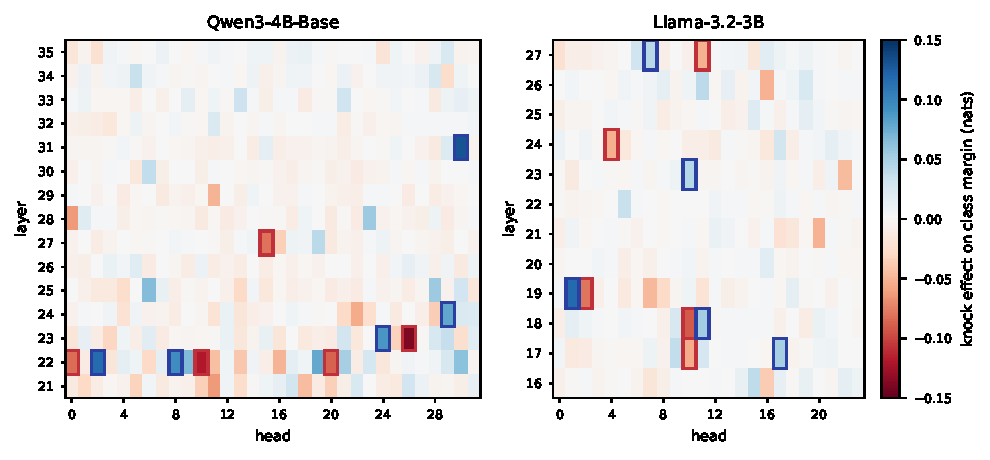
\includegraphics[width=\linewidth]{figures/fig17_headgrid.pdf}
\caption{No single head carries the answer. Effect on the 12-shot class margin of knocking one head at the query position (mean over 144 prompts from six label families; blue lowers the margin, red raises it; colour clipped at $\pm0.15$ nats), for every head in the reader layers of Qwen3-4B-Base (layers 21--35) and Llama-3.2-3B (layers 16--27). Outlined cells are the five most negative and five most positive heads. The largest single-head effects are $-0.14$ nats (Qwen L23h26, a query head) and $+0.13$ (Qwen L31h30, a brake), and $-0.09$ / $+0.12$ in Llama (L18h10, L19h1), against a 1.3-nat margin; the sets built from these rankings move the margin by $-0.74$ and $+1.39$ (Qwen) and $-0.56$ and $+1.90$ (Llama) when knocked together (Table~\ref{tab:claims}).}
\label{fig:headgrid}
\end{figure}

The readers are about ninety heads, and about two dozen heads work against them. Neither number is an accident of our search; the model uses many heads where a few would seem to do, and the arithmetic below says why.

A reader, concretely, is an upper-layer head whose attention from the arrow prefers slots whose class matches the query. Twenty readers chosen on one draw of prompts and knocked out together on a fresh draw cost $-0.74$ \ci{-0.95}{-0.55} nats; twenty random heads from the same layers cost $+0.02$. No single reader is necessary: the largest single-head knock in Qwen costs 0.09. Against the readers stand the brakes, twenty-four heads in layers 22--34 that write against the label the model has just seen. Knocking them on a fresh draw raises the margin by $+1.39$ \ci{+0.88}{+1.88}, nearly tripling it; twenty-four random heads give $+0.22$. The brakes are negative heads in the sense of the indirect-object circuit's negative name movers and of copy suppression: they take a label that is being copied and push the logits the other way.

What the brakes buy is calibration. Permuting the order of the demonstrations leaves the mean margin unchanged but moves single prompts by more than a nat on half of them, and the readers themselves are recency-biased, with a gradient of 0.5--0.85 nats from the first slot to the last. With the brakes removed the model follows that gradient and prefers whichever label came last. At six demonstrations the brakes carry the anti-recency term outright; at twelve they hold the model order-neutral against the readers' pull. Figure~\ref{fig:populations} shows the reader--brake interaction and the order effect.

Why populations? One might think the model spreads the read over ninety heads because no single head can tell the classes apart. The attention rows say otherwise. A single reader's class bias is 0.2--0.4 nats against a per-slot spread of about 0.5, so one head already separates the classes in its own attention pattern, if weakly. What no head has is output gain.

\begin{proposition}[Gain bound]\label{prop:gain}
Let head $i$ attend with mass $m_i$ to slots whose values differ by $\Delta v$ between the two labels, with output-value matrix $W_{OV}^{(i)}$, and let $w$ be the final-norm-scaled unembedding direction of the correct minus the alternative label. The head's direct contribution to the margin is at most $m_i\,\|W_{OV}^{(i)}\Delta v\|\,\|w\|/\rho$, where $\rho$ is the RMS scale of the final residual. If the margin $M$ is carried by the heads' direct contributions and every head's bound is at most $\beta$, at least $\lceil M/\beta \rceil$ heads contribute.
\end{proposition}

Measured, no head in Qwen writes more than 0.2 nats of the answer logit directly (Section~\ref{sec:accounting}), so a 1.3-nat class flip needs at least seven heads; the model uses 14 for half of it and 46 for 80\%. Gain forces the populations; missing signal does not. We characterize them instead by the direction they read and write and test that direction against random subspaces. Searching for a single responsible head would look for something the arithmetic says cannot exist. The same arithmetic predicts that knocking the seven largest direct movers in the copier band should remove 0.3--0.5 of the $+0.68$ twelve-demonstration margin. It removed $-0.16$ \ci{-0.56}{+0.24}: the predicted sign, smaller than predicted, with an interval that includes zero. We count it as weak support.

\begin{figure}[t]\centering
\fig{figures/fig6_populations.pdf}
\caption{Readers and brakes act as populations with opposite signs. (a) Joint knock of 20 readers, 24 brakes, and both, on a fresh draw, against size-matched random sets (grey). (b) Order effect: margin against the position of the last matching demonstration, intact and with brakes knocked.}
\label{fig:populations}
\end{figure}

\section{Does it add up? Exact accounting and validation}\label{sec:accounting}
The sections so far locate each step by the change it causes. We can also ask a stricter question of a single prompt: which components wrote the answer's logit, and how much each. The residual stream before the final norm is a sum over components, so the answer logit decomposes exactly.

\begin{proposition}[Direct decomposition]\label{prop:dla}
Let $x = e + \sum_i a_i + \sum_l m_l$ be the final residual at the arrow, with $e$ the embedding, $a_i$ the head outputs and $m_l$ the MLP outputs, and let $\rho = \mathrm{rms}(x)$. With $w = \gamma \odot W_U^\top(\mathbf 1_{y} - \mathbf 1_{y'})$ for the final-norm gain $\gamma$ and labels $y, y'$, the margin is $\mathrm{logit}(y) - \mathrm{logit}(y') = \big(w^\top e + \sum_i w^\top a_i + \sum_l w^\top m_l\big)/\rho$.
\end{proposition}

The proposition is an identity, and we use it as a check: on every prompt the right-hand side, computed from the hooked components, agrees with the model's own margin with a mean error of 0.045 nats in Qwen and 0.048 in SmolLM3. The decomposition then says who writes the answer. On intact twelve-demonstration prompts the margin is $+0.68$ nats; attention in layers 30--35 contributes $+0.66$, attention in layers 21--29 $+0.14$, and the late MLPs $-0.11$. Under the exact class flip the answer swings by $-1.33$: the layer 30--35 band moves by $-1.12$, the readers by $-0.36$, and the late MLPs the other way, by $+0.25$. The readers, then, are the source of the answer and not its writer. They collect the label values into the arrow; a band of copier heads in the last six layers reads that and writes the logits; the final MLPs act as a prior toward the label seen most and oppose the flip. Fourteen heads carry half the direct swing and 46 carry 80\% in Qwen; eight and 45 in SmolLM3. Figure~\ref{fig:waterfall} shows the decomposition as a waterfall and Figure~\ref{fig:accounting} the per-head concentration curve. The direct accounting assigns nats to the last writer; the handoffs of the previous sections assign them to the source. Together they close the path from slot to logit.

\begin{figure}[t]\centering
\fig{figures/fig7_accounting.pdf}
\caption{Every nat of the answer assigned to a component. (a) Direct contributions to the margin by layer band, intact and under the class flip, Qwen and SmolLM3. (b) Cumulative share of the flip against number of heads, sorted by contribution.}
\label{fig:accounting}
\end{figure}

\begin{figure}[t]\centering
\fig{figures/fig9_waterfall.pdf}
\caption{The answer as a sum of bands. Left: the intact twelve-demonstration margin in Qwen, built up band by band; the layer 30--35 copier band writes almost all of it. Right: the change under the exact class flip; the copier band carries most of the swing, the readers a quarter, and the late MLPs push the other way.}
\label{fig:waterfall}
\end{figure}


\paragraph{Faithfulness, completeness, minimality.} \citet{wang2022ioi} ask three things of a circuit. Faithfulness: the exact decomposition above is an accounting identity, not a faithfulness test. The real test is to keep only the named heads at the query (writers, duplicate-token, pooling, query, reader, brake and copier heads, 67 in all, with the late MLPs) and replace every other head's output there by a reference value. The reference matters. With means taken over natural text the named set keeps nothing ($-0.79$ / $-0.88$ nats from an intact $+1.13$ / $+0.55$, rare / symbol labels), but so does a random set of the same size ($-0.83$ / $-0.79$) and so does keeping no heads at all ($-0.82$ / $-0.81$): a thousand heads replaced by a value 2.5 times further from their own output than the battery mean push the query residual off anything the late layers have seen, and the test stops ranking. With \citet{wang2022ioi}'s reference, the mean over a matched distribution, the test ranks. Matched has to mean matched on the label pair as well: the battery stores each prompt under two label pairs, and a reference that mixes them, or a resample partner that is the same prompt under the other pair, moves the numbers by up to a nat in either direction (Section~\ref{sec:transfer}). All values below use the mean over same-pair prompts at the query, or a resampled same-pair prompt. With the named set plus the eight heads a screen of layers 20--27 adds (Appendix~\ref{app:complete}; 79 heads), the circuit alone keeps about 60\% of the margin on both label kinds (resample: $-0.28$ [$-0.50,-0.09$] of $+0.55$ on symbol labels, $-0.47$ of $+1.14$ on rare ones; a random set of about the same size drawn from the same layers $-0.65$ / $-0.98$, no heads $-0.69$ / $-0.95$), and the complement cut one band at a time says where the rest is: layers 0--19 $-0.16$ / $-0.29$, layers 20--27 $-0.07$ / $-0.10$, layers 28--35 $+0.09$ / $+0.17$ (removing the unnamed late heads helps; they are net brakes). The natural-label study of Section~\ref{sec:transfer} then adds 110 heads, readers and brakes that matter when the label is a word, and with that final set (189 heads) the circuit alone is above intact on both label kinds ($+0.89$ / $+1.26$ under resample, $+0.93$ / $+1.62$ with the mean reference; random $-0.64$ / $-0.98$), the two late bands help when their remaining heads go ($+0.40$ / $+0.99$ and $+0.35$ / $+0.65$) and only the encoder band still costs ($-0.07$ / $-0.17$). Within the layers where the mechanism lives, the circuit is complete, and the same protocol closes it in SmolLM3-3B and Llama-3.2-3B as well (Appendix~\ref{app:complete}). Completeness in the selection sense: every named set was selected on one draw of prompts and tested on a fresh draw against random sets of the same size and layers (readers $-0.74$ against $+0.02$; brakes $+1.39$ against $+0.22$; the Llama sets $+1.90$ and $-0.56$ against $+0.12$ and $0.00$), so the sets carry their function on prompts they were not chosen on. Minimality is where the account departs from a sparse circuit. No single reader or brake is necessary in the intact network: the largest single-head knock in Qwen costs 0.09 nats and in Llama 0.12. \citet{wang2022ioi}'s criterion is weaker than this, since it lets a head count as necessary once the others are removed, and we have not run that conditional test; what Proposition~\ref{prop:gain} rules out is a single head carrying a 1.3-nat answer when no head writes more than 0.2 nats. We report populations with their direction-level tests in place of a minimal head set, and say so wherever it applies.

\subsection{Cutting the arrows}\label{sec:arrows}
The interventions above establish the parts. The arrows between them were, until this point, inferred from the parts coexisting. Four further experiments cut the arrows directly, each on fresh prompt draws in Qwen3-4B (Table~\ref{tab:arrows}).

\paragraph{Readers hand to the late layers.} Take the concept battery and its class-flipped twin, and hand the twenty readers' outputs at the query from the twin into the intact run. This carries $-1.08$ nats of the twin's $-1.80$ on rare-word labels and $-0.54$ of $-0.95$ on symbol labels: sixty percent of everything that differs between the two prompts passes through those twenty heads. Then hold the inputs of every attention head in layers 30--35 at their intact values while the readers' outputs still come from the twin: the effect drops to $-0.81$ and $-0.35$. Hold the inputs of the layer 30--35 MLPs as well: $-0.39$ and $-0.19$. So of what the readers write, a quarter to a third is read by late attention heads (the copiers), about forty percent by late MLPs, and the remaining third goes straight to the logits. The arrow from readers to copiers is cut and measured; it is one of three routes out of the readers, not the only one.

\paragraph{The gate acts partly through the readers' queries.} Knock the sixteen duplicate-token heads and add the gate direction $g$ back at layer 23 of the query. On unique-label prompts, where the gate is closed, this opens it: the margin rises by $+0.58$ nats at one unit of $g$ and $+0.90$ at two, and the sharp reader 29:11 moves its mass off the sink (0.91 to 0.37). Now remove the direction $g$ from the twenty readers' query inputs alone, leaving it everywhere else. The rise falls to $+0.43$ and $+0.61$, and 29:11's sink mass climbs back (0.37 to 0.51; 0.35 to 0.62); removing a random direction of the same kind from the same queries changes nothing ($+0.58$, $+0.92$, sink mass unchanged). A quarter to a third of what $g$ does to the answer travels through the readers' queries, the route the account draws; the rest reaches the answer through heads and MLPs we have not named. On recurring prompts the same knock lowers $g$ from $+18$ to $+13$ and costs $0.28$ nats; adding one unit of $g$ brings the margin back to within $0.04$ of intact.

\paragraph{Turning up a few readers does not replace the rest.} If the readers are many only because no single head can write enough (Proposition~\ref{prop:gain}), amplifying a few should do the work of all. Multiply the attention output of three readers (24:21, 29:11, 22:20) at the query by two, on prompts drawn with a seed not used to choose them: the margin rises $+0.40$ (rare) and $+0.25$ (symbols), against $+0.04$ for three random heads. By four it still rises; by eight it breaks ($-0.56$, $-0.84$). Knock the other seventeen readers and the margin falls $-0.89$ and $-0.50$; amplifying the three by four on top recovers only to $-0.46$ and $-0.44$, and by eight makes it worse. Three heads turned up cannot stand in for seventeen. The gain bound is a bound, and the readers' writes do add, but the other heads carry information the three do not have. Why training spread the computation remains open.

\paragraph{Position zero is a working sink, not an empty one.} Qwen and SmolLM3 add no beginning-of-sequence token, so position zero holds the prompt's first word. Zeroing its value for the reader layers costs $0.33$ nats on unique-label prompts and nothing measurable ($-0.03$) on recurring ones, with the same operation on position one costing nothing in either case. Zeroing it at every layer removes the sink altogether (the readers put no mass there), and the margin falls by $0.76$ and $0.43$. The position does the sink's job; its content is not the point, but it is not absent either.


\paragraph{The same cuts in SmolLM3 and Llama.} The two arrow experiments were repeated on fresh draws in SmolLM3-3B and Llama-3.2-3B with their own reader and duplicate-head sets and their own fitted gate directions (Table~\ref{tab:arrows_rep}). The readers' handoff replicates in both: SmolLM3's twenty readers carry the whole class-flipped twin effect ($-2.16$ against the twin's $-2.05$ on rare-word labels, $-1.52$ against $-1.30$ on symbols; random sixteen heads $-0.11$ / $-0.07$), and Llama's twenty carry 45\% / 54\% of it ($-0.86$ of $-1.92$, $-0.46$ of $-0.86$). The route after the readers differs by family. In SmolLM3, as in Qwen, holding the late attention inputs (L30--35) at their intact values removes 36\% of the handoff and holding the late MLP inputs as well removes another 27\%, leaving 37\% that reaches the logits directly. In Llama the holds remove nothing ($-0.86 \to -1.02 \to -1.09$): its readers reach the logits without a late relay. The gate-to-query route replicates in all three. Adding $g$ at the query opens the gate in every family ($+0.53$ / $+0.69$ nats in SmolLM3 with and without the duplicate heads knocked, $+0.64$ / $+0.92$ in Llama), and removing $g$ from the readers' queries takes back 12--46\% of that in SmolLM3 and 37--79\% in Llama, growing with the dose, while a random direction of the same norm takes back nothing ($+0.68$, $+0.91$). The step before the gate does not replicate as a margin effect. Knocking the sixteen duplicate-token heads moves the gate projection in every family and in the direction the circuit predicts (unique-label prompts: $+1.8$ units in SmolLM3, $+4.5$ in Llama; recurring: $-0.7$, $-2.4$), but in SmolLM3 and Llama the margin does not fall with it ($+0.90$ and $-0.39$, against Qwen's clean closure), because those heads also carry other things the knock removes. The arrow from the duplicate heads into $g$ is shown at the level of the gate feature in all three models and at the level of behaviour in Qwen only.

\paragraph{Where the rest of $g$ goes.} With the readers' queries carrying a third to a half of $g$'s effect, we swept the remainder in Qwen: remove $g$ from every head's queries in a band of layers, or from the MLP inputs in a band, with the gate direction added at layer 23 and the duplicate heads knocked. Removing it from all queries in L23--35 takes back as much as removing it from the twenty readers alone ($+0.34 \to +0.18$ in both cases), and the band-by-band values (L23--26 $+0.35$, L27--30 $+0.13$, L31--35 $+0.33$) say that the query-side route runs through the middle band where the readers sit. Removing $g$ from MLP inputs changes nothing specific ($+0.25$ to $+0.51$ across bands, random direction $+0.32$). The other half of $g$'s effect is not a second named route through MLPs but is carried by the same reader queries in a way the direction removal does not reach, or by heads outside the twenty that read $g$ weakly each; we cannot tell these apart with this design.

\paragraph{A cleaner sink test.} Zeroing position zero's value for every other position's reads while leaving its own residual stream untouched costs $0.34$ nats on unique-label prompts and $0.05$ on recurring ones in the reader layers ($0.50$ and $0.05$ at every layer), against $0.33$ and $0.03$ for the ordinary zeroing. The sink's effect on the readers is in its value as read by others; what the all-layer zeroing added ($0.76$ against $0.50$) came from position zero's own stream. Swapping position zero's value for another prompt's costs $1.50$ nats, so the value is not inert: it is the content the readers fall back on.

\begin{table}[t]
\centering\small
\caption{The arrow cuts in SmolLM3-3B and Llama-3.2-3B, fresh draws. Change in answer margin (nats) from intact, mean over prompts; concept battery rare / symbol ($n=71$ each), slotgate ($n=60$). The hold columns fix the inputs of the late attention and MLP layers (SmolLM3 L30--35, Llama L22--27) at their intact values.}\label{tab:arrows_rep}
\begin{tabular}{llrr}
\toprule
Intervention & Battery & SmolLM3 & Llama \\
\midrule
Class-flipped twin, everything & concept & $-2.05$ / $-1.30$ & $-1.92$ / $-0.86$ \\
\quad twenty readers' outputs from twin & concept & $-2.16$ / $-1.52$ & $-0.86$ / $-0.46$ \\
\quad\quad + hold late attention inputs & concept & $-1.38$ / $-1.24$ & $-1.02$ / $-0.61$ \\
\quad\quad + hold late attention and MLP inputs & concept & $-0.79$ / $-0.53$ & $-1.09$ / $-0.52$ \\
\quad random sixteen heads from twin & concept & $-0.11$ / $-0.07$ & $-0.16$ / $+0.05$ \\
\midrule
Twenty readers knocked / random twenty & slotgate & $-1.32$ / $-0.05$ & $-0.13$ / $+0.23$ \\
Duplicate heads knocked & slotgate & $+0.90$ & $-0.39$ \\
$g$ at the query ($\times 1$) & slotgate & $+0.53$ & $+0.64$ \\
\quad + duplicate heads knocked & slotgate & $+0.69$ & $+0.92$ \\
\quad\quad $g$ removed from readers' queries & slotgate & $+0.61$ & $+0.48$ \\
\quad\quad random direction removed & slotgate & $+0.68$ & $+0.91$ \\
\bottomrule
\end{tabular}
\end{table}

\begin{table}[t]
\centering\small
\caption{Four interventions on connections, Qwen3-4B-Base, fresh draws. Change in answer margin (nats) from intact, mean with 95\% bootstrap interval over prompts. Concept battery: rare-word / symbol labels ($n=72$ each); slotgate: unique / recurring label prompts ($n=30$ each).}\label{tab:arrows}
\begin{tabular}{llr}
\toprule
Intervention & Battery & $\Delta$ margin \\
\midrule
Class-flipped twin, everything & concept & $-1.80$ / $-0.95$ \\
\quad twenty readers' outputs from twin & concept & $-1.08$ / $-0.54$ \\
\quad\quad + hold attention inputs L30--35 & concept & $-0.81$ / $-0.35$ \\
\quad\quad + hold attention and MLP inputs L30--35 & concept & $-0.39$ / $-0.19$ \\
\midrule
Duplicate heads knocked & slotgate & $+0.15$ / $-0.28$ \\
\quad + $g$ at layer 23 ($\times 1$) & slotgate & $+0.58$ / $+0.04$ \\
\quad + $g$, $g$ removed from readers' queries & slotgate & $+0.43$ / $-0.06$ \\
\quad + $2g$ & slotgate & $+0.90$ / $+0.12$ \\
\quad + $2g$, $g$ removed from readers' queries & slotgate & $+0.61$ / $-0.08$ \\
\quad + $2g$, random direction removed from readers' queries & slotgate & $+0.92$ / $+0.13$ \\
\midrule
Three readers $\times 2$ / random three $\times 2$ & concept & $+0.40$, $+0.04$ / $+0.25$, $+0.03$ \\
Other seventeen readers knocked & concept & $-0.89$ / $-0.50$ \\
\quad + three readers $\times 4$ & concept & $-0.46$ / $-0.44$ \\
\midrule
Position 0 value zeroed, L21--29 / position 1 & slotgate & $-0.33$, $-0.01$ / $-0.03$, $+0.02$ \\
Position 0 value zeroed, all layers & slotgate & $-0.76$ / $-0.43$ \\
\bottomrule
\end{tabular}
\end{table}

\section{Three models, one algorithm}\label{sec:replication}
Should three models trained by three groups on three corpora run the same algorithm? Not in every detail, and it helps to say in advance which details are free. Some parts of the account follow from attention itself: a softmax over positions has to put its mass somewhere, some position must serve as the sink, and a key written into a label token can only be read through that token's keys. Those parts should appear in any transformer that does the task, and if a fourth model lacked them we would count the account falsified. Other parts are choices that training makes: which heads do each job, how many of them, how strong the gate is, in which layers the work happens. Those we expect to differ, and we report them as the model's implementation of the algorithm. A link counts as replicated when the same intervention has the same sign with an interval that excludes zero and the matched control inside noise; we do not ask the magnitudes to agree, and they differ by up to a factor of three.

By this standard the account replicates in SmolLM3-3B and Llama-3.2-3B. The slot's value and key dissociate in both (Section~\ref{sec:slot}). The read law fits 124 of 125 Llama slot-reading heads and predicts the one-slot regime more tightly than in Qwen. The null action exists in both. The implementation differs in ways worth recording. Llama's readers sit in layers 14--27 of 28 where Qwen's sit in 21--29 of 36. Llama's gate is weaker: 67\% of its unique-label prompts still receive a label, against 10\% in Qwen. The heads a generic induction score selects act as a withholding population there. They hold the mid-layer readers in the sink, and ablating them raises the margin by about a nat (Figure~\ref{fig:gatemodels}). Where Qwen has two nameable query computers, SmolLM3 and Llama spread the query computation. And where Qwen's 24 brakes stand out in a single-head census, Llama's do not: a census of all 288 Llama heads found no head whose knock moves the margin by more than 0.12 nats, 271 of them within $\pm 0.03$. Yet the sets exist. The 24 heads the census ranks as brakes, knocked together on a fresh twelve-demonstration draw, raise the margin by $+1.90$ \ci{+1.12}{+2.67} against $+0.12$ for 24 random heads, and the 20 heads it ranks as readers cost $-0.56$ \ci{-1.01}{-0.12} against $0.00$. At six demonstrations, where Llama's margin is only $+0.40$, the brake set gives $+0.57$ \ci{+0.19}{+0.93} against $+0.16$ and the reader set is not detectable. Llama has the same two populations as Qwen, each weak head by head and strong as a set.

The algorithm also assembles in a fixed order during training. Across OLMo-2 checkpoints the copy of a repeated label appears first, the null action second, and the readers' class selectivity last; the 1B model never develops the readers, which is why it does not do the task. The order is the one the dependencies require: nothing can be gated before there is something to copy, and nothing can be matched by class before the keys are written (Figure~\ref{fig:olmo}, Appendix~\ref{app:olmo}).

\begin{table}[t]\centering\small
\caption{Each link of the account in three models. Forced: follows from the architecture and is expected in every model. Implementation: set by training and reported per model. Named: a small set of heads is necessary and sufficient. Population: no single head is necessary; the link is characterized by a direction with a size-matched random control. --: not run.}
\label{tab:replication}
\begin{tabularx}{\linewidth}{Yllll}
\toprule
Link & Kind & Qwen3-4B & SmolLM3-3B & Llama-3.2-3B \\
\midrule
Slot value (label) at label-token V & forced & yes & yes & yes \\
Slot key (class) at label-token K, mid layers & forced & yes & yes & yes \\
Writers, dose spread across depth & implementation & population & population & -- \\
Read law within regime / down-transfer & forced & 127/140, 0.07 & 7/8 & 124/125, 0.04 \\
Read law up-transfer (18 demos) & tested & failed & -- & failed \\
Duplicate detector feeds gate & implementation & named & yes & weak \\
Gate lowers null logit, not match & forced (sign) & yes & yes & -- \\
Query code & implementation & named & population & -- \\
Readers (source) & forced (population) & population & population & population \\
Brakes & implementation & 24 heads & suppressors & 24-head set, $+1.90$ \\
Value transport & implementation & 3 groups & -- & -- \\
Direct writer = late band & implementation & yes & yes & -- \\
Order term sign flip 6 vs 12 & implementation & yes & yes (3 carriers) & -- \\
\bottomrule
\end{tabularx}
\end{table}

\begin{figure}[t]\centering
\fig{figures/fig10_gate_models.pdf}
\caption{The null action in two families. (a) Llama-3.2-3B emits a label on 67\% of unique-label prompts, Qwen3-4B on 10\%: the same fallback, gated far more weakly. (b) In Qwen, pushing the gate signal $g$ at its natural dose lowers the sink logit relative to the matching slots at the three strongest readers (red) and moves matching against the other slots by much less (grey). (c) In Llama, knocking the sixteen heads a generic induction score selects moves the mid-layer readers' mass out of the sink and onto the slots: there the induction-scored heads hold the read closed.}
\label{fig:gatemodels}
\end{figure}

\section{Does the circuit carry other tasks, and labels that mean something?}\label{sec:transfer}
The circuit was found on batteries whose classes are surface regularities and whose labels are arbitrary tokens. A mechanism worth the name should carry retrieval when the class is a real semantic feature and when the labels are words with meanings of their own. We built one more battery to ask this (\texttt{concept12n}): four concepts a reader would call natural (topic: animal vs.\ food; language: English vs.\ Spanish; question vs.\ statement; implied sentiment: good vs.\ bad), twelve demonstrations each, and the same prompt written four ways that differ only in the two label words: arbitrary symbols (\texttt{foo}/\texttt{bar}), rare words (\texttt{zorp}/\texttt{quil}), the concept's own words (\texttt{animal}/\texttt{food}), and those words exchanged, the flipped labels of \citet{wei2023larger}. 384 prompts per model, the same named sets as Section~\ref{sec:replication}, and the same interventions, with predictions written before the data (Appendix~\ref{app:claims}).

\paragraph{Arbitrary labels transfer.} With symbol and rare labels on the natural concepts the named parts carry retrieval in all three families: circuit-only with a resampled reference is at intact in Qwen3-4B ($-0.05$ and $+0.96$ nats relative to intact for symbol and rare labels) and below it but far above a random set of the same size and layers in Llama ($-0.58$ / $-0.11$; random $-1.5$ / $-1.3$) and SmolLM3 ($-0.82$ / $-0.47$, intervals reaching zero; random $-1.6$ / $-1.5$); with the mean reference all three are at or above intact. With the final sets of this section (189, 122 and 163 heads) the symbol battery of Section~\ref{sec:accounting} gives the same answer in all three: $+0.89$ / $+1.26$ (Qwen), $+0.87$ / $+1.01$ (SmolLM3) and $+0.03$ / $+0.75$ (Llama) relative to intact under resample, against $-0.64$ / $-0.98$, $-0.71$ / $-1.11$ and $-0.26$ / $-0.71$ for random sets. The retrieval stage does not care what the class is.

\paragraph{Meaningful labels split the margin in two.} With the concept's own words as labels the intact margin triples ($5.4$ nats in Qwen and SmolLM3, $4.9$ in Llama). Because each prompt appears once with the natural labels and once with them exchanged, the two margins can be added and subtracted: half their sum is the part that follows the demonstrations ($R$), half their difference the part that follows what the words mean ($P$). In all three models the two are of the same size ($R\approx2.7$--$2.9$, $P\approx2.2$--$2.7$ nats), which is why flipped labels end near zero in a 3--4B base model, as \citet{wei2023larger} reported behaviourally. The meaning part is not the circuit's: removing the MLPs outside the named late ones costs $3.8$ nats on natural labels against $1.1$ on symbols, and removing the late unnamed heads, the brakes, \emph{helps} the flipped prompts ($+0.4$ nats in SmolLM3 and Llama), as predicted: the prior enters through the late band and the circuit's readers have to win against it.

\paragraph{The retrieval part needs more readers when the label is a word.} The named sets carry a quarter to a half of $R$ on natural labels (Qwen $-2.16$ of $2.86$ nats, SmolLM3 $-1.50$ of $2.67$, Llama $-1.44$ of $2.71$; reference matched on label pair and label set, see below). The band test puts the remainder in the reader and copier layers, not in a new place, and the per-head screen on the natural-label prompts names it. In Qwen 73 heads outside the set in layers 16--27 cross $-0.03$ nats, the largest of which (24:30, 27:18, 24:26, 26:4) put 0.4--0.7 of their attention on the slots whose label matches the answer; a second screen of layers 28--35, which the symbol-label screen had declared closed, finds 37 more, two of them slot-attending readers (33:30, 29:14) and the rest sink-attending copiers and brakes. In Llama 52 heads at layers 11--16, its writer and first-reader stage; in SmolLM3 15 heads, nine of them in layers 14--17 and six in 30--31. They attend the same way on symbol prompts, where they barely matter: the slot-reading stage is a population whose active membership depends on what has to be copied, and a word like \emph{animal} can be moved to the logits by many more heads than an arbitrary token can. With the screened heads added (Qwen 189 heads, Llama 163, SmolLM3 122; Figure~\ref{fig:closure}) circuit-only on natural labels is within the intact interval under resample ablation in Qwen ($-0.16$ nats of $2.87$, interval $[-0.71,+0.38]$; random set $-2.89$, no heads $-3.12$) and keeps 86\% and 81\% of $R$ in Llama and SmolLM3 under the mean reference ($-0.39$, $-0.51$; random $-2.4$, $-2.8$). Under the mean reference Qwen overshoots ($+0.97$) and its word-meaning part rises by $2.8$ nats, and in all three models removing the unnamed late heads raises $P$ by about $+2$ nats: what is left outside the set at those layers is brakes, and the prior they hold down is the word's meaning. Every layer band from the readers on is closed in all three (Qwen 28--35 $+1.13$, SmolLM3 30--35 $-0.01$, Llama 22--27 $-0.20$); what SmolLM3 and Llama still lose sits in the encoder band (SmolLM3 layers 0--17 $-0.56$, with only nine heads crossing the single-head threshold there), the same diffuse substrate as on arbitrary labels. Our predictions before the late screen were that at most ten heads would cross and that the 28--35 complement would be neutral; both were wrong, and the misses are what taught us that the brake population grows with the label's meaning.

\begin{figure}[t]\centering
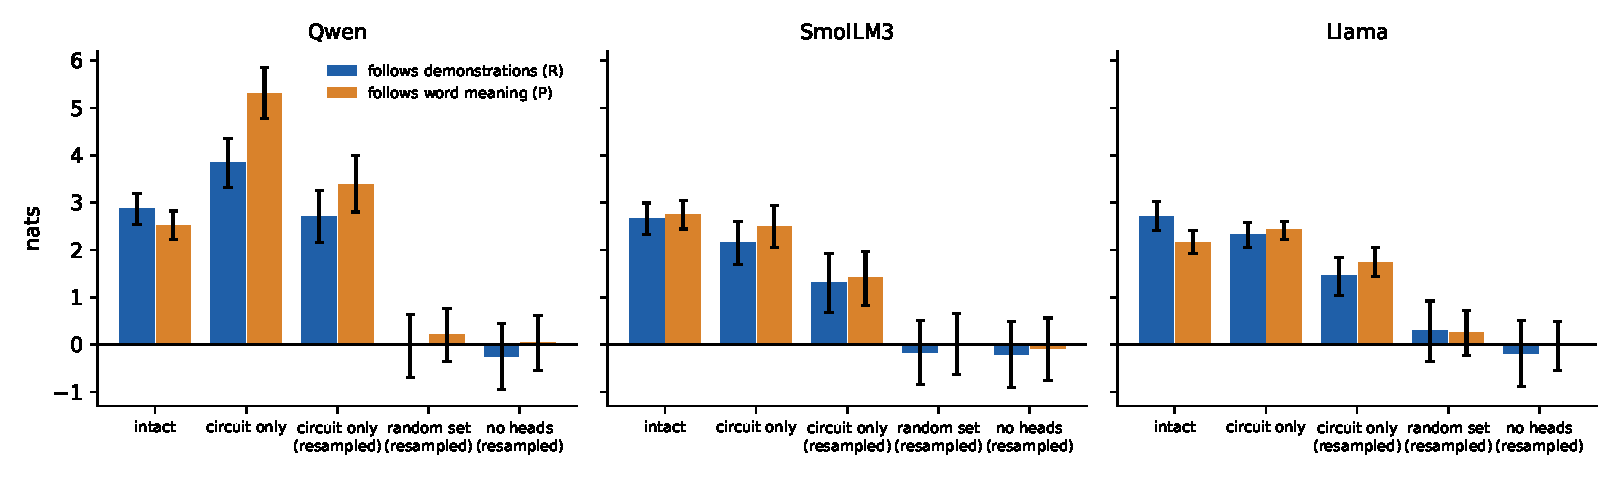
\includegraphics[width=\textwidth]{figures/fig21_closure.pdf}
\caption{Natural-label closure. For each model, the part of the margin that follows the demonstrations ($R$, blue) and the part that follows what the label words mean ($P$, orange) intact and with only the named heads kept at the query (final sets: 189, 122 and 163 heads with the late MLPs), the reference being the mean over same-kind prompts or a resampled same-kind prompt; against a random set of the same size and layers, and against no heads. Bars are means over 96 natural/flipped prompt pairs; whiskers are 95\% bootstrap intervals.}
\label{fig:closure}
\end{figure}

\paragraph{Why resampling is harsher on words.} Under resample the circuit-only margin is $0.5$--$0.9$ nats lower than under the mean reference on natural labels, and not on symbols. The resample partner is another prompt of the same kind, whose answer is the other label half the time, so this only costs if the unnamed heads carry answer evidence; on word labels they do (the screen's unnamed effects sum to $-10$ nats against $-3$ for the named heads) and on symbols they do not. A word like \emph{animal} can be moved to the logits by many weak heads; an arbitrary token only by the few readers that copy anything. On word labels the reader stage is a population whose active membership depends on what has to be copied, and completeness is a statement about that population.

\paragraph{A control we got wrong first.} The batteries store each prompt several times in a row, once per label set, and our first resample control took its reference from the next prompt; the mean reference averaged over all the label pairs of the battery. On this battery the next prompt of a natural-label prompt is the same sentences with the labels exchanged, so the control injected the opposite mapping; on the symbol battery of Section~\ref{sec:accounting} it is the same sentences under the other invented pair, the same mapping, which can only help. The bias has no fixed sign: when the reference was matched on label set (mean over same-kind prompts, partner the next prompt of the same kind) one result here reversed (SmolLM3 carrying $R$ with its original set), Qwen's symbol-battery circuit-only fell from $+0.49$ to $-0.28$, and SmolLM3's and Llama's rose. Every number in this paper that compares a circuit-only run with intact now uses the matched reference; Appendix~\ref{app:complete} keeps the one superseded value with its explanation.

\section{Does size change the parts, and does post-training keep them?}\label{sec:scale}
Everything so far was measured in base models of three to four billion parameters. Two questions a reader will ask next have known behavioural answers and, until now, no mechanistic one. \citet{wei2023larger} found that only large models follow flipped labels: a small model answers with what the label word means, a large one with what the demonstrations say. And post-training is where every deployed model lives. We ran the same census in the Qwen3 family at 0.6B, 1.7B, 4B and 8B parameters, and the Qwen3-4B instruct model with the base model's heads, with the predictions written down first (Appendix~\ref{app:claims}). Each size got its own census: head identities and the gate direction were never carried from one size to another.

\begin{figure}[t]\centering
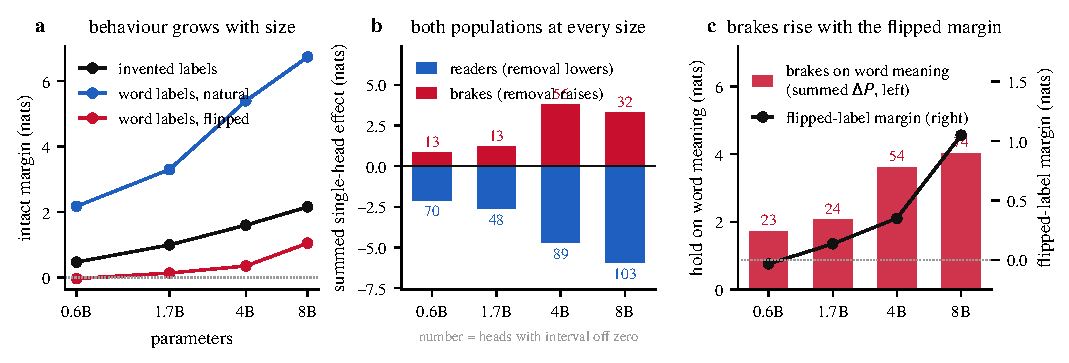
\includegraphics[width=\textwidth]{figures/fig23_scale.pdf}
\caption{One census at four sizes (Qwen3 base 0.6B, 1.7B, 4B, 8B). (a) Intact margins for invented labels, natural word labels and flipped word labels. (b) Reader and brake populations: summed effect of the heads whose single removal at the query lowers (blue) or raises (red) the margin with the interval off zero; the number is the head count. (c) The summed hold of the brakes on word meaning (bars, left axis) against the flipped-label margin (line, right axis): the two rise together.}\label{fig:scale}
\end{figure}

\begin{figure}[t]\centering
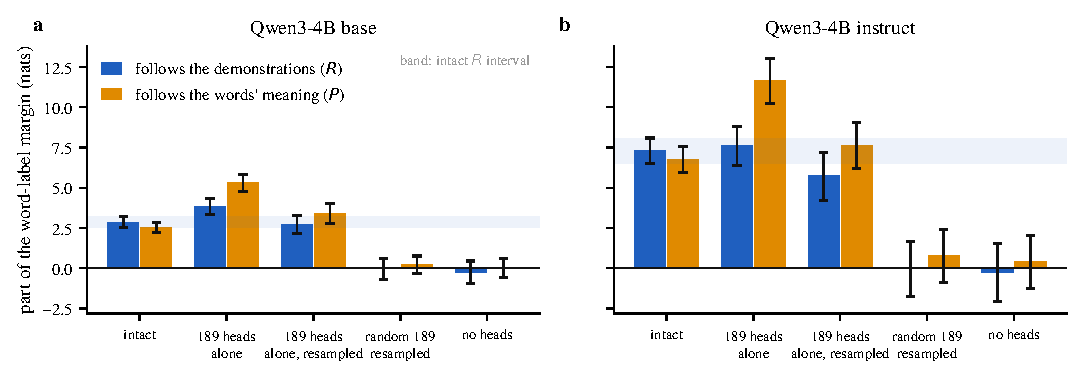
\includegraphics[width=\textwidth]{figures/fig22_instruct.pdf}
\caption{Qwen3-4B base (a) and instruct (b) on the word-label prompts, the base model's 189 heads in both. Blue: the part of the margin that follows the demonstrations ($R$); orange: the part that follows the words' meaning ($P$); the band is the intact $R$ interval. Post-training multiplies both parts by about 2.5 and keeps their ratio; the 189 heads alone, resampled reference, keep 79\% of $R$ in the instruct model, and a random set of the same size keeps none.}\label{fig:instruct}
\end{figure}

\paragraph{The same parts at every size.} The census screens every head in the upper half of the model (layers 10--27 of 28 at 0.6B and 1.7B, 16--35 of 36 at 4B and 8B) by removing it alone at the query on the \texttt{concept12n} battery, with the per-kind mean as reference. At every size there is a reader population, heads whose removal lowers the margin with the interval off zero, and a brake population, heads whose removal raises it. Table~\ref{tab:scale} and Figure~\ref{fig:scale} give the counts and the summed effects. The readers' summed effect grows with size, from $-2.1$ nats at 0.6B to $-5.9$ at 8B. The brakes' summed effect grows from $+0.8$ through $+1.2$ to $+3.8$ at 4B and then falls back to $+3.3$ at 8B, where fewer heads cross the interval (32 against 56); we had predicted a monotone rise, and that part missed. The largest single reader, as a fraction of the intact margin, shrinks from 22\% to 18, 18 and 15\%: a bigger model spreads the read over more heads, which is what the gain bound of Section~\ref{sec:read} predicts when the margin to be produced grows faster than one head's output can. One thing we did not predict: within a layout the parts sit at the same addresses. The two 28-layer models share their top brake, 22:7 ($+0.27$ and $+0.43$ nats), their second, 26:7, and nine reader positions; the two 36-layer models share their five strongest readers (29:11, 24:29, 28:0, 24:30, 24:22) and their five strongest brakes (25:30, 28:23, 31:30, 25:14, 33:21). Whether that is initialisation, data order or something about the task we cannot say from these runs.

\paragraph{The gate exists, and acts, at every size.} For each size we fitted the gate direction from its own unique- versus recurring-label prompt pairs (Section~\ref{sec:gate}). It separates held-out pairs perfectly at every layer of the upper half in all four models, and its relative size at the arrow peaks in the last third of the stack in all four (layer 22 of 28 at 0.6B and 1.7B, 23 of 36 at 4B, 24--34 of 36 at 8B). Adding the fitted direction at the query arrow of unique-label prompts, at the dose the model itself uses, raises their label margin by $+1.75$ (0.6B), $+0.95$ (1.7B) and $+1.11$ (8B) nats; at 4B, where the intact unique-label margin is already $+0.24$, the single dose gives $+0.25$ with an interval reaching zero and the double dose $+0.78$. A random direction of the same norm moves it by at most $0.2$ in the wrong direction. Taking the direction away from recurring-label prompts lowers theirs by $1.35$, $0.69$, $0.72$ and $1.07$ nats at single dose (0.6B, 1.7B, 4B, 8B), $2.9$, $1.7$, $1.8$ and $3.0$ at double. Two predictions failed: that a single dose would clear zero at every size (4B did not), and that the double dose would beat the single one everywhere (at 8B they tie, $1.10$ against $1.11$; the add side saturates there while the remove side still doubles).

\paragraph{Where the flipped-label curve comes from.} The paired natural and flipped prompts give, at every size, the part of the margin that follows the demonstrations ($R$) and the part that follows the words ($P$). Both grow with size, but $R$ grows faster: $P/R$ falls from $1.03$ at 0.6B through $0.92$ and $0.88$ to $0.73$ at 8B, and the flipped-label margin rises from $-0.03$ through $+0.14$ and $+0.35$ to $+1.05$ nats. That is the curve of \citet{wei2023larger} inside one family, and the census says what moves it. The brakes on word meaning, the heads whose removal raises $P$, hold down $1.7$ nats at 0.6B, $2.1$ at 1.7B, $3.6$ at 4B and $4.0$ at 8B (23, 24, 54 and 74 heads), and that sum is the one quantity in the census that rises in step with the flipped-label margin at every size; the reader population that carries $R$ grows alongside. The gate does not track size this way: its dose effect is of the same order at every size (Table~\ref{tab:scale}), so the gate is a part present everywhere, not the lever that moves the curve. A small model's readers and its word-meaning prior are matched in strength, so exchanging the labels cancels the demonstrations; a large model's readers out-pull the prior, and the brakes it has grown hold the prior down further. Two details of our prediction missed: we expected the 1.7B flipped margin to be negative (it is $+0.14$, interval crossing zero) and the 0.6B rare-label margin below $0.3$ nats (it is $0.62$). The monotone parts of the predictions held.

\paragraph{Post-training keeps the circuit and turns up the brakes.} Qwen3-4B instruct has the same architecture as its base, so the base model's 189-head set can be left untouched in it with no re-identification. It carries retrieval: on the symbol battery the heads alone, resampled reference, are at or above intact ($+0.43$ / $+1.29$ nats relative to intact for symbol and rare labels; base $+0.89$ / $+1.26$), a random set of the same size and layers loses $0.66$ / $1.15$, and removing the 189 heads costs exactly what removing every head costs ($-0.61$ / $-1.00$ against $-0.60$ / $-1.00$). The base model's gate direction, not refitted, is positive at layer 23 on all 144 prompts. What post-training changed is the gain (Figure~\ref{fig:instruct}). With word labels both parts of the margin are about $2.5$ times larger ($R=7.30$, $P=6.75$; base $2.87$ and $2.52$) and their ratio is unchanged ($0.92$ against $0.88$), so the instruct model still half-follows meaning on flipped labels, as \citet{wei2023larger} reported for instruction-tuned models. We had predicted $P$ up and $R$ flat; the data say both. The extra gain on meaning is held down by the unnamed heads of layers 16--27, whose removal now raises $P$ by $4.9$ nats (base: about $2$), and the 189 heads keep 79\% of $R$ (base: all of it). Post-training did not rewire the readers; it added braking in the population around them.

\begin{table}[t]\centering\small
\caption{One census, four sizes (Qwen3 base, \texttt{concept12n}, 384 prompts each, upper-half heads removed one at a time at the query). Readers: removal lowers the margin, interval off zero; brakes: removal raises it. $R$ and $P$ are the demonstration-following and meaning-following parts of the word-label margin. Gate dose: change in unique-label margin when the size's own fitted direction is added at the query arrow at the model's own dose and at twice it, and change in recurring-label margin when it is taken away. 0.6B and 1.7B screen layers 10--27 (288 heads), 4B and 8B layers 16--35 (640 heads).}\label{tab:scale}
\begin{tabularx}{\linewidth}{Yrrrr}
\toprule
 & 0.6B & 1.7B & 4B & 8B \\
\midrule
Intact margin, symbol / rare labels (nats) & 0.32 / 0.62 & 0.87 / 1.12 & 1.62 / 1.57 & 2.43 / 1.88 \\
Natural / flipped word labels & 2.18 / $-0.03$ & 3.30 / $+0.14$ & 5.40 / $+0.35$ & 6.74 / $+1.05$ \\
$R$ / $P$ & 1.07 / 1.10 & 1.72 / 1.58 & 2.87 / 2.52 & 3.90 / 2.85 \\
Readers: count, summed effect & 70, $-2.08$ & 48, $-2.60$ & 89, $-4.69$ & 103, $-5.94$ \\
Largest reader, \% of intact & 22 & 18 & 18 & 15 \\
Brakes: count, summed effect & 13, $+0.82$ & 13, $+1.21$ & 56, $+3.76$ & 32, $+3.27$ \\
Brakes on word meaning: count, summed $\Delta P$ & 23, $+1.73$ & 24, $+2.06$ & 54, $+3.61$ & 74, $+4.03$ \\
Gate dose on unique-label margin, single / double & $+1.75$ / $+1.96$ & $+0.95$ / $+1.71$ & $+0.25$ / $+0.78$ & $+1.11$ / $+1.10$ \\
Gate removed from recurring-label prompts, single / double & $-1.35$ / $-2.87$ & $-0.69$ / $-1.68$ & $-0.72$ / $-1.80$ & $-1.07$ / $-3.02$ \\
\bottomrule
\end{tabularx}
\end{table}

\section{Building it from parts}\label{sec:build}
A mechanism found by cutting should also be buildable. We did this twice: once by writing the weights of a small transformer by hand to be exactly the circuit of Figure~\ref{fig:algorithm}, and once by training a small transformer from scratch on the task and looking for the parts.

\paragraph{Hand-set weights.} The toy is attention-only with three layers and a residual stream of named blocks (class direction, label identity, position, token type, duplicate flag, gate, slot key, query code). Layer 1 holds the writers, which attend from each label token back to its sentence and copy the class into the slot-key block, and from the query arrow back to its sentence into the query-code block, together with a duplicate detector that marks a label token whose identity appeared before. Layer 2 holds one pooling head that averages the duplicate flags over the label positions into the gate block at the arrow. Layer 3 holds the readers, whose query is the query code plus the gate, whose keys are the slot keys and one fixed sink key at position 0, and whose values are the label identities, read out by the unembedding. Nothing is trained. On the slotgate prompts the toy reproduces Proposition~\ref{prop:law} exactly (largest deviation $10^{-16}$, since the law is the softmax it was built from) and the gate phenomenology of Section~\ref{sec:gate}: on unique-label prompts the sink takes 0.67 of the readers' mass and the margin is $+0.24$; adding $g$ empties the sink and raises it to $+0.73$. On recurring-label prompts (margin $+0.83$, sink 0.02) knocking the duplicate detector sends 0.54 of the mass to the sink ($+0.39$), adding $g$ back rescues it ($+0.84$), and removing $g$ from the readers' queries undoes the rescue ($+0.39$). Knocking the writers leaves nothing to read ($0.00$). Capping each reader's output as Proposition~\ref{prop:gain} does makes the margin grow with the number of readers (0.16, 0.49, 1.25, 2.53 nats for 1, 3, 8, 20 heads). This is a sufficiency result: these parts, wired this way, produce the law and the gate. It says nothing yet about whether a trained model chooses them.

\paragraph{Trained from scratch.} We trained a four-layer, eight-head Llama-architecture model (hidden size 256, 3.4M parameters) on a synthetic version of the task: 48 word tokens each carrying two of eight latent classes, sentences of three words sharing exactly one class, 32 arbitrary label tokens redrawn every prompt, and prompts of two to six demonstrations followed by a query. Two training distributions, three seeds each: a mix of unique-label and recurring-label prompts, and recurring-label prompts only. The task is learned abruptly between 8k and 30k steps; at 40k steps every run answers both prompt kinds with a margin near 10 nats. The parts we could look for with the same loupes are there: swapping a slot's residual at the writer layers moves the answer by 7--11 nats in every seed, and class-flip attribution finds one or two reader heads in the last layer (a small model needs no population; its single heads clear the gain bound). The gate is not there in either distribution. The direction separating unique- from recurring-label prompts at the arrow has held-out sign accuracy of 0.45--0.62 in all six runs, steering along it does nothing consistent, and unique- and recurring-label prompts are answered with the same margin (8.8--10.7 nats). Looking back, this is what the account predicts: the toy has no prior to fall back on and its unique-label mapping is always consistent, so retrieving is always right and nothing selects for a gate. The gate in the pretrained models exists because a set of unique labels does not certify a consistent mapping against the language prior. The matching test is a third training distribution in which every unique-label prompt carries a fresh, unpredictable query label, so that recurrence is the only certificate that retrieval will pay. Four of five seeds learned the task, and in all four the gate appears. Recurring-label prompts are answered with a margin of 8.7--9.1 nats and unique-label ones with 1.8--2.3 (in the other two distributions both kinds get 8.8--10.7). The recurring-minus-unique direction at the arrow in layer 2 is decodable held-out at 0.81--1.00 (0.54--0.60 in the controls), and steering along it by one natural gap moves the answer: pushing a recurring prompt toward ``unique'' drops its margin from 9 to 0.7 and 1.1 in two seeds (a random direction of the same norm: 7.0 and 5.8), pushing a unique prompt toward ``recurring'' raises it from 2.3 to 8.0 in one seed and from 2.0 to 4.0 in another (random: 1.8 and 0.9); which side is steerable varies by seed (Appendix~\ref{app:toy}). In the mixed and recurring-only controls the same push changes nothing (margins move by less than 0.1). A gate forms when, and only when, unique-label retrieval is penalised in training, which is the first causal answer to why the pretrained models have one.

\section{Related work}\label{sec:related}
\paragraph{What in-context learning computes.} One line of work asks what function few-shot ICL implements, abstracting from the network. \citet{garg2022functions} train transformers to learn simple function classes in context, and \citet{akyurek2022linear} and \citet{vonoswald2022gd} show that, for linear regression, the computation can be read as gradient descent or ridge regression carried out by attention. These results describe the input--output map on synthetic tasks. We study a pretrained model on text, and ask which heads carry out which step; the answer we find is a lookup in a memory, with no step that resembles a gradient update.

\paragraph{Label tokens and the ICL circuit.} \citet{cho2024circuit} give a three-step skeleton of an ICL inference circuit in which label tokens store task information that a later head reads. \citet{zheng2024labelwords} and \citet{hu2025addition} identify label words as the local carriers of that information. We add what the slot holds on which side of attention, who writes it and at what depth, and what switches the read on. \citet{kim2025schema} dissociate task schema from binding; our dissociation is at the level of a single label token's keys and values. \citet{jiao2026conflict} study what happens when demonstrations conflict; the brakes we describe are the population that decides which of two recent labels wins.

\paragraph{Task vectors and induction heads.} \citet{hendel2023taskvectors} and \citet{todd2023fv} extract a task or function vector from a few heads' outputs at the query. Our query code is the same kind of object seen from its consumers: two heads write it, and it lives in the span of the readers' match functionals, not in any one reader's weight-space probe. \citet{olsson2022induction} established induction heads as the copying mechanism of in-context learning and the phase change in which they appear. Our duplicate-token detectors are the first half of that circuit put to a second use: they produce the repeat signal that the gate pools. The readers are induction heads whose match is on a class feature; the emergence order we observe extends the induction-head phase change by two further stages. \citet{yu2024qk} locate recency in query--key similarity to label positions; we find the same bias in the readers' rows and the population that cancels it.

\paragraph{Negative heads and the attention sink.} \citet{wang2022ioi} found negative name-mover heads that write against the answer, and \citet{mcdougall2023copysuppression} describe copy suppression as a general function of such heads. Our brakes are a population with that sign and a measurable job, calibration against recency. \citet{xiao2023sinks} describe the attention sink as a position that absorbs mass; we give it a function in retrieval, as the null position whose logit the gate controls.

\paragraph{Methods.} Activation patching descends from causal mediation analysis~\citep{vig2020mediation} and the locating experiments of \citet{meng2022rome}; \citet{hanna2023greaterthan} and \citet{nanda2023grokking} use it to recover full circuits for arithmetic tasks. \citet{wang2022ioi} evaluate a circuit by faithfulness, completeness and minimality; our exact accounting is a per-prompt faithfulness check, and our population results are where minimality fails for a reason we can state. \citet{quirke2026stress} stress-test attribution with same-answer controls, which we adopt throughout. \citet{chen2024skillpath} and the objection that ``circuit'' bundles sparsity, localisability and modularity~\citep{bricken2026notcircuits} frame the question our component-or-population split answers (Appendix~\ref{app:populations}).

\section{Discussion}\label{sec:discussion}
What the account covers is narrow and we want the boundary visible. It covers two-class label retrieval and function selection with short sentences and single-token labels, at up to twelve demonstrations, in three base models of three to four billion parameters, with the parts and the gate re-found at four sizes of one family (Section~\ref{sec:scale}) and the base model's heads still carrying retrieval after post-training. It does not cover instruction following, long-form tasks, or many-class binding, and the sizes stop at 8B. Within that boundary, every link has an intervention and a control; outside it we have not looked.

Two predictions did not hold, and both taught us something. The read law does not extrapolate to longer prompts. Empirically a head's null mass and its total matching mass stay roughly constant as matching slots are added, so the added slots share what was there; the law we fitted at twelve demonstrations had absorbed this saturation into its constants. We describe this and do not yet explain it: the fitted parameters are not separately identifiable ($n_{\mathrm{rest}}$ and $e^{L_{\mathrm{sink}}}$ enter only through their sum), so the stability is a fact about the heads that needs its own account. We also expected that fine-tuning on many-shot prompts, where recency costs accuracy, would strengthen the brakes; 400 steps of LoRA moved the readers' necessity threefold and left the brakes where they were ($+1.32$ against $+1.44$ nats). Where the brakes come from in training is open. A third test, the knock of the seven largest direct movers, had the predicted sign and an interval that includes zero.

The split between named components and populations is, we think, the most general lesson. Where the model needs little gain it concentrates: two heads compute the query's class, sixteen detect repeats, three value groups carry most of the label identity. Where it needs output gain beyond what one head's $W_{OV}$ provides, it sums, and no head is necessary. The populations are still circuits in the ordinary sense: they have a definite input direction, a definite output direction, and those directions are specific against random subspaces of the same dimension. What they lack is a single responsible head, and the arithmetic of Proposition~\ref{prop:gain} says why one cannot exist. An account of a transformer behavior should say, for each step, whether the model concentrated or summed, and give the population-level object where it summed. This is also our answer to the worry that ``circuit'' presupposes sparsity: the sparsity is decided step by step by the gain the step requires.

The null action deserves a last word. A model that reads a prompt memory needs a way to not read it, and the softmax provides one for free: a position that every head can fall back on. In Qwen and SmolLM3 that position holds the prompt's first token, so it is a learned role rather than an empty slot; removing its value at every layer leaves the readers nowhere to put unspent mass, and unique-label prompts, where not reading is the right action, get worse by 0.4--0.8 nats. We suspect this is why attention sinks are universal, and why the gate acts on the readers' queries and nowhere else. It is the one place a prompt-level signal can reach the only lever there is.

\section*{Reproducibility}
Code, batteries, the per-prompt measurement hooks and the scripts that produce every figure and table are released at \url{https://github.com/andrewgcodes/in-context-learning-circuit}. All runs used single H100s with the HuggingFace implementations of the models in bfloat16.

\bibliographystyle{iclr2024_conference}
\bibliography{refs}

\appendix
\section{Batteries, interventions and statistics}\label{app:setup}
\paragraph{Batteries.} Full sentence pools, label sets and seeds are in the released code. The concept battery draws three demonstrations per class from two pools of a given axis; concept12 six per class; slotgate two per class with a token-identical unique-label twin; manyclass $K$ classes from six pools (positive, negative, animals, food, Spanish, questions) with $12/K$ (or $18/K$) demonstrations per class and arbitrary single-token labels.
\paragraph{Statistics.} All intervals are paired bootstraps over prompts (4000 resamples). Head sets selected on a battery were confirmed on a fresh draw of prompts from the same pools with a different seed. Random controls match the number of heads and their layers.
\paragraph{Tokenization.} Targets are scored as full token sequences; the first token of a two-token label carries the key. Llama's tokenizer prepends a beginning-of-sequence token that the prompt-side comparison strips.
\section{Table of effects}\label{app:claims}
Every number in the main text with its model, $n$ (prompts) and paired-bootstrap interval.
{\scriptsize
\begin{xltabular}{\linewidth}{>{\hsize=.72\hsize}Y l r >{\hsize=1.28\hsize}Y}
\caption{Effects behind the main text (nats; paired against the intact run; 95\% bootstrap intervals).}\label{tab:claims}\\
\toprule
Claim & Model & $n$ & Effect [95\% CI] \\
\midrule
\endfirsthead
\multicolumn{4}{l}{\textit{Table \ref{tab:claims} continued}}\\
\toprule
Claim & Model & $n$ & Effect [95\% CI] \\
\midrule
\endhead
\midrule\multicolumn{4}{r}{\textit{continued on next page}}\\
\endfoot
\endlastfoot
Label exchange: K/V at all positions, reader layers & Qwen & 144 & $-7.15$ [$-7.39,-6.90$] \\
Label exchange: label-token K/V, all layers (= full twin) & Qwen & 144 & $-7.18$ [$-7.43,-6.94$] \\
Label exchange: 8 readers' V / K & Qwen & 144 & $-2.16$ [$-2.41,-1.90$] / $+0.56$ [$+0.44,+0.69$] \\
Label exchange: label-token K/V, all layers (= full twin) & Llama & 144 & $-4.92$ [$-5.31,-4.55$] \\
Label exchange: label-token K/V, all layers (= full twin) / L21--29 & SmolLM3 & 144 & $-5.55$ [$-5.93,-5.15$] / $-2.94$ [$-3.30,-2.58$] \\
Sentence swap: twin & Qwen & 176 & $-2.87$ [$-3.13,-2.62$] \\
Sentence swap: label K/V L21--29 & Qwen & 176 & $-2.35$ [$-2.58,-2.12$] \\
Sentence swap: 8 readers' K / V & Qwen & 176 & $-0.55$ [$-0.67,-0.44$] / $+0.10$ [$+0.07,+0.14$] \\
Sentence swap: label K/V by band & Llama & 432 & $-0.02$, $-0.15$, $-0.15$, $-0.04$ (twin $-0.23$) \\
Sentence swap: query attention by band & Llama & 432 & $-0.03$, $-0.18$, $-0.13$ \\
Sentence swap: exact span & SmolLM3 & 432 & $-0.33$ [$-0.41,-0.25$] \\
Same-class twin (control) & Qwen & 168 & $+0.08$ [$-0.07,+0.23$] / $+0.08$ \\
Spread (4 layers) vs single-layer dose, natural / double & SmolLM3 & 144 & $+0.56$ [$+0.48,+0.65$] vs $+0.37$ [$+0.29,+0.46$] / $+0.69$ [$+0.58,+0.81$] vs $+0.20$ [$+0.09,+0.31$] \\
Gate signal, recurring / unique & Qwen & 30/30 & $+18.3$ / $-20.9$ \\
Gate signal, 16 duplicate heads off & Qwen & 30/30 & $-0.3$ / $-19.1$ (random16 $+17.5$ / $-21.3$; induction16 $+14.0$ / $-7.4$) \\
$+g$: null $-$ match logit & Qwen & 30 & $-1.75$ [$-1.94,-1.55$] / $-3.25$ / $-3.65$; random $+0.17$ / $-0.17$ / $-0.19$ \\
$+g$: match $-$ other logit & Qwen & 30 & $+0.47$ / $+0.34$ / $+0.48$; random $-0.04$ / $+0.05$ / $+0.03$ \\
Query code: pair handoff & Qwen & 144 & $-0.53$ [$-0.68,-0.39$] (exact twin $-1.33$) \\
Query code: hold attn 24--29 / 24--35 & Qwen & 144 & $-0.14$ [$-0.17,-0.10$] / $-0.04$ [$-0.06,-0.03$] \\
Query code: hold attn+MLP / MLP 30--35 & Qwen & 144 & $-0.01$ / $-0.66$ [$-0.83,-0.50$] \\
Readers 21--29 attention out & Qwen & 144 & $-1.10$ [$-1.39,-0.82$] \\
Reader-20 knock, fresh draw & Qwen & 144 & $-0.74$ [$-0.95,-0.55$] / $+0.02$ \\
Brake-24 knock, fresh draw & Qwen & 144 & $+1.39$ [$+0.88,+1.88$] / $+0.22$ \\
Top-7 direct movers knock & Qwen & 144 & $-0.16$ [$-0.56,+0.24$] / $-0.02$, $+0.13$, $+0.05$ \\
Brake-24 after many-shot / few-shot LoRA & Qwen & 144 & $+1.32$ [$+0.81,+1.82$] / $+1.44$ [$+0.86,+2.01$] \\
Read law within regime & Qwen, Llama & 96 & 127/140, 124/125 heads within 0.1 \\
Read law, one slot per class & Qwen, Llama & 96 & median error 0.07 / 0.04 \\
Read law, 18 demonstrations & Qwen, Llama & 96 & median error 0.15 / 0.13 (failed) \\
Exact accounting & Qwen, SmolLM3 & 144 & recon.\ error 0.045 / 0.048; 14/46 and 8/45 heads \\
Llama single-head census & Llama & 144 & max reader $-0.09$, max brake $+0.12$, random-288 joint $+0.74$ \\
Census-ranked brake-24 / reader-20 joint knock, 12 demos & Llama & 144 & $+1.90$ [$+1.12,+2.67$] (random $+0.12$) / $-0.56$ [$-1.01,-0.12$] (random $0.00$) \\
Census-ranked brake-24 / reader-20 joint knock, 6 demos & Llama & 432 & $+0.57$ [$+0.19,+0.93$] (random $+0.16$) / $-0.06$ [$-0.32,+0.21$] \\
\midrule
Instruct, 189 base heads only (resampled) vs intact, symbol / rare & Qwen3-4B instruct & 144 & $+0.43$ [$-0.17,+1.01$] / $+1.29$ [$-0.08,+2.69$] (random $-0.66$ / $-1.15$) \\
Instruct, 189 heads removed / all heads removed & Qwen3-4B instruct & 144 & $-0.61$ / $-1.00$ vs $-0.60$ / $-1.00$ \\
Instruct, word labels: $R$ / $P$ intact & Qwen3-4B instruct & 96 & $+7.30$ [$+6.49,+8.09$] / $+6.75$ [$+5.92,+7.55$] \\
Instruct, 189 heads only (resampled): $\Delta R$ / $\Delta P$ & Qwen3-4B instruct & 96 & $-1.53$ [$-3.07,-0.11$] / $+0.88$ [$-0.57,+2.29$] (random $-7.29$ / $-5.98$) \\
Instruct, unnamed heads L16--27 removed: $\Delta R$ / $\Delta P$ & Qwen3-4B instruct & 96 & $-0.27$ / $+4.93$ \\
Gate dose $+g$ at query, unique-label prompts, single / double & Qwen3-0.6B & 30 & $+1.75$ [$+1.57,+1.95$] / $+1.96$ [$+1.68,+2.24$]; random $-0.13$ / $-0.26$ \\
 & Qwen3-1.7B & 30 & $+0.95$ [$+0.68,+1.18$] / $+1.71$ [$+1.33,+2.08$]; random $+0.02$ / $-0.07$ \\
 & Qwen3-4B & 30 & $+0.25$ [$-0.14,+0.62$] / $+0.78$ [$+0.32,+1.25$]; random $-0.08$ / $-0.34$ \\
 & Qwen3-8B & 30 & $+1.11$ [$+0.79,+1.43$] / $+1.10$ [$+0.57,+1.63$]; random $+0.09$ / $+0.20$ \\
Gate removed at query, recurring-label prompts, single / double & Qwen3 0.6B / 1.7B / 4B / 8B & 30 & $-1.35$ / $-2.87$; $-0.69$ / $-1.68$; $-0.72$ / $-1.80$; $-1.07$ / $-3.02$ \\
Census, intact symbol / rare / natural / flipped & Qwen3 0.6B / 1.7B / 4B / 8B & 384 & 0.32 / 0.62 / 2.18 / $-0.03$; 0.87 / 1.12 / 3.30 / $+0.14$; 1.62 / 1.57 / 5.40 / $+0.35$; 2.43 / 1.88 / 6.74 / $+1.05$ \\
Census, readers: count, summed effect & Qwen3 0.6B / 1.7B / 4B / 8B & 384 & 70, $-2.08$; 48, $-2.60$; 89, $-4.69$; 103, $-5.94$ \\
Census, brakes: count, summed effect & Qwen3 0.6B / 1.7B / 4B / 8B & 384 & 13, $+0.82$; 13, $+1.21$; 56, $+3.76$; 32, $+3.27$ \\
Census, brakes on word meaning: count, summed $\Delta P$ & Qwen3 0.6B / 1.7B / 4B / 8B & 96 pairs & 23, $+1.73$; 24, $+2.06$; 54, $+3.61$; 74, $+4.03$ \\
Gate fit, held-out sign agreement & Qwen3 0.6B / 1.7B / 8B & 23 pairs & 1.00 at every layer 6--27 / 6--27 / 10--35 \\
\bottomrule
\end{xltabular}}
\section{Encoder bound and assembly from parts}\label{app:encoder}
The encoder bound is correlational: every axis that failed to bind (parity, third letter, letter set, digit rules) is one the model never represents linearly at the arrow at any layer, while language becomes linear by layer 8 and binds weakly through layers 10--20, and topic, sentiment and implied meaning become linear by layer 13 and bind through layers 21--29. Adding the gate to a non-binding prompt changes nothing. Assembly from parts: writing the task direction $u$ into the query-class slots at layer 16 and at the query of a parity prompt raises accuracy from 50\% to 71\% (question 38\%$\to$58\%, vowel 50\%$\to$71\%), with key-only, query-only and random directions within $\pm0.1$ and the wrong-class slots hurting; SmolLM3 reproduces this at a model-specific dose. The same-answer control: handoffs from a same-class same-length twin move the answer by at most 0.06 nats.
\section{Why the all-layer label-token handoff must reproduce the swap}\label{app:induction}
Let two prompts $A$ and $B$ have the same length and identical tokens except at a set of positions $S$ (here the label tokens). Run the model on $B$ and, at every layer, replace the keys and values computed at the positions in $S$ by those from the run on $A$. We claim that every position outside $S$ then carries exactly its $A$-run residual stream at every layer, so the logits at the query equal those of prompt $A$.

The proof is an induction over layers. At the input, positions outside $S$ have the same token in $A$ and $B$, so their embeddings agree. Suppose that at the input of layer $\ell$ every position outside $S$ agrees with the $A$ run. Attention at such a position reads its own query (which agrees), and keys and values from every position: those outside $S$ agree by the hypothesis, and those inside $S$ have been replaced by the $A$ run's. So the attention output agrees, the MLP, which acts position-wise, agrees, and the residual stream at the output of layer $\ell$ agrees. The query position is outside $S$, so its final residual and its logits are those of $A$. Nothing in the argument uses what the model has learned; it holds for a randomly initialised transformer and for any choice of $S$, including a set of positions that carries no task information at all. The reviewer who pointed this out to us checked it on random transformers with and without query-key normalisation.

So the exact recovery in Section~\ref{sec:slot} tells us only that the harness patches what it says it patches. The informative handoffs are the ones the theorem does not cover: keys and values at the label tokens in a band of layers, values without keys, keys without values, and a changed sentence transmitted through the keys at positions where the input did not change.

\section{Order effects and the many-shot fine-tuning test}\label{app:order}
The order of the demonstrations should not matter to a model that has stored them in a memory, and on average it does not: permuting the twelve demonstrations leaves the mean margin unchanged. Single prompts move, by more than a nat on half of them. The readers are the source of the movement. Their attention rows favor late slots, with a gradient of 0.5--0.85 nats of logit from the first slot to the last, so a prompt whose last matching demonstration sits near the query is read more strongly than one whose matching demonstrations come early. The brakes cancel this. With the 24 brakes knocked out the model prefers whichever label came last; at six demonstrations the brakes carry the anti-recency term outright, and at twelve they hold the model order-neutral against the readers' pull. In SmolLM3 three heads carry most of the order term and can be named.

We predicted that fine-tuning on many-shot prompts, where recency costs accuracy, would strengthen the brakes. It did not. We trained two LoRA adapters on Qwen3-4B (rank 16, $\alpha = 32$, learning rate $10^{-4}$, 400 steps, adapters on every linear layer) on axes disjoint from the test battery, one on many-shot prompts and one on few-shot prompts, so that the arms differ only in demonstration count. After training, knocking the 24 brakes raises the margin by $+1.32$ \ci{+0.81}{+1.82} in the many-shot arm and $+1.44$ \ci{+0.86}{+2.01} in the few-shot arm: the same brakes, the same gain. The readers moved instead; their knock cost rose about threefold under adaptation in both arms. Whatever sets the brakes' strength, 400 steps of many-shot training is not it.

\section{Emergence across OLMo-2 checkpoints}\label{app:olmo}
\begin{figure}[t]\centering
\fig{figures/fig11_olmo.pdf}
\caption{The circuit assembles in order during training. Across OLMo-2 stage-1 checkpoints (grey: 1B; black: 7B), copying a repeated label is present from the earliest checkpoint; the null action, measured as withholding a label on unique-label prompts, appears in 1B between 315B and 839B tokens and is already present at 42B in 7B; class-keyed retrieval, measured as a positive margin on unique-label prompts, arrives last, by 630B tokens in 7B and never in 1B. Thirty prompts per point.}
\label{fig:olmo}
\end{figure}

OLMo-2 releases intermediate checkpoints, which let us ask in what order the parts of the circuit appear. We ran the slotgate battery (two labels used twice against four labels used once, thirty prompts each) on six stage-1 checkpoints of OLMo-2 1B (10k, 50k, 150k, 400k, 900k and 1.9M steps; 21B to 4T tokens) and five of OLMo-2 7B (10k to 929k steps; 42B to 3.9T tokens), and read three measures at each. Copying a repeated label is present from the first checkpoint in both models: on recurring prompts the label is the argmax at every checkpoint, and knocking the sixteen duplicate-token heads removes the recurring margin from the first checkpoint on (1B at 10k steps: $+0.11$ to $-1.96$). The null action comes second. In 1B, the share of unique-label prompts that still receive a label is 0.63, 0.73 and 0.60 at the first three checkpoints and 0.13, 0.03 and 0.17 at the last three, so withholding appears between 315B and 839B tokens; in 7B it is already 0.17 at 42B tokens. Class-keyed retrieval comes last. The unique-prompt margin in 1B is negative at every checkpoint ($-3.5$ to $-0.5$) and the model never does the task; in 7B it turns positive by 630B tokens ($+0.86$, accuracy 0.67; $+0.72$ at 3.9T). The order copy, then null action, then readers is the one the dependencies require. Two observations are specific to immature checkpoints: in trained 1B and in early 7B, knocking the duplicate-token heads raises label emission on unique prompts (1B: 0.17 to 0.73), the opposite sign to Qwen; the trained 7B has Qwen's sign. We also ran Pythia-1.4B across six checkpoints; it is at chance on the task at every one and tells us nothing about the order.

\section{Example prompts}\label{app:prompts}
One verbatim prompt per battery as the Qwen tokenizer sees it (the query sentence is held out of the demonstrations; the model is scored on the next token after the final arrow).

\paragraph{Twelve demonstrations, invented words (concept12)} 149 tokens; target \texttt{quil}, alternative \texttt{zorp}.
\begin{quote}\small\ttfamily
kludom trolom blidom -> quil\\
tratak grodak gridak -> zorp\\
prunom trogom plutom -> quil\\
drobak klirak vrirak -> zorp\\
blitom frelom klumom -> quil\\
sturak grupak grodak -> zorp\\
klemak tramak blirak -> zorp\\
vromak snibak stenak -> zorp\\
dropom snukom plapom -> quil\\
plisom vrebom drapom -> quil\\
frelak prirak gripak -> zorp\\
pribom vredom vremom -> quil\\
grinom blorom skedom ->
\end{quote}
\paragraph{Four demonstrations, labels repeat (slotgate, recurring member)} 45 tokens; target \texttt{foo}, alternative \texttt{bar}.
\begin{quote}\small\ttfamily
The omelet was folded over melted cheese -> foo\\
a wonderful, heartfelt film -> bar\\
an absolute joy to read -> bar\\
The pancakes were stacked with syrup -> foo\\
The steak rested before it was sliced ->
\end{quote}
\paragraph{Four demonstrations, every label once (slotgate, unique member; token-identical to the recurring member except the two late labels)} 45 tokens; target \texttt{foo}, alternative \texttt{bar}.
\begin{quote}\small\ttfamily
The omelet was folded over melted cheese -> foo\\
a wonderful, heartfelt film -> bar\\
an absolute joy to read -> vex\\
The pancakes were stacked with syrup -> baz\\
The steak rested before it was sliced ->
\end{quote}
\paragraph{Three classes, four demonstrations each (manyclass)} 121 tokens; target \texttt{foo}, alternative \texttt{vex}.
\begin{quote}\small\ttfamily
cold food and a long wait -> vex\\
a wonderful, heartfelt film -> lux\\
Which road leads to the harbor -> foo\\
charming and genuinely funny -> lux\\
What time does the pharmacy close -> foo\\
Should we take the highway or the coast road -> foo\\
buggy, slow and badly designed -> vex\\
wooden acting and a lazy script -> vex\\
cozy room with a great view -> lux\\
the worst concert I have seen -> vex\\
a warm and moving story -> lux\\
Where did you leave the car keys -> foo\\
How long does the bread need to rise ->
\end{quote}


\section{Trained toy: the gate condition}\label{app:toy}
Three training distributions for the 3.4M-parameter toy of Section~\ref{sec:build}, all with arbitrary labels redrawn per prompt: \emph{mix} (half the prompts unique-label with a consistent query label, half recurring-label), \emph{recurring-only}, and \emph{gate} (half recurring-label; the other half unique-label prompts whose query label is drawn fresh from the labels not used in the demonstrations, so that retrieval is never rewarded on a unique-label prompt). Runs of 40k steps (mix, recurring-only) or 80k steps (gate; one 40k gate seed that learned is also shown), three to five seeds each; one gate seed did not learn the task and is excluded. Margins are over 160 held-out prompts per kind.

\begin{table}[h]\centering\small
\begin{tabular}{llcccccc}
\toprule
training & seed & unique & recurring & direction & recurring $\to$ unique & unique $\to$ recurring \\
\midrule
mix & 0 & 8.8 & 8.8 & 0.60 & 8.9 (8.8) & 8.7 (8.7) \\
recurring-only & 0 & 10.3 & 10.4 & 0.54 & 10.4 (10.4) & 10.2 (10.3) \\
gate & 0 & 1.8 & 9.1 & 0.93 & \textbf{0.7} (7.0) & 1.8 (1.5) \\
gate & 1 & 2.3 & 9.0 & 1.00 & \textbf{1.1} (5.8) & \textbf{8.0} (1.8) \\
gate & 4 & 2.0 & 8.7 & 0.99 & 8.1 (7.1) & \textbf{4.0} (0.9) \\
gate & 2$^{\dagger}$ & 2.0 & 8.7 & 0.81 & 7.3 (8.2) & 2.9 (1.9) \\
\bottomrule
\end{tabular}
\caption{The gate forms only when unique-label retrieval is penalised. ``Unique'' and ``recurring'' are intact margins in nats (correct label against the best other demonstrated label) on held-out prompts of each kind. ``Direction'' is the held-out sign accuracy of the mean-difference direction between recurring- and unique-label prompts at the query arrow after layer 2 (chance 0.5). The last two columns steer along that direction by one natural gap at the arrow in layer 2 and report the resulting margin, with a random direction of the same norm in parentheses: recurring prompts pushed toward ``unique'', and unique prompts pushed toward ``recurring''. Bold: the steer moves the margin by more than 3 nats further than its random control. Mix and recurring-only: one seed shown; the other seeds have direction accuracy 0.43--0.61 and are reported in the released logs. $^{\dagger}$40k steps.}
\label{tab:toygate}
\end{table}

In the gate runs the same slot and reader parts are present as in the other two (slot swap at the writer layers moves the answer by 9 nats; one or two last-layer readers carry the class-flip attribution), so the gate is added to an otherwise unchanged mechanism rather than replacing it. Steering is partial and seed-dependent: in two seeds the direction closes the gate (recurring prompts lose 8 nats against 2--3 for a random push), in two it opens it (unique prompts gain 2--6 nats against none), and no seed is fully steerable both ways at this dose. The direction is a real and necessary part of the open signal but not all of it, which matches what we found for $g$ in the pretrained models (Section~\ref{sec:arrows}). The earlier draft of this test used a fixed push of $0.5\sqrt{d}$, which is several natural gaps in this small model; at that dose a random direction collapses the margin too, so the dose must be set from the measured gap.

\paragraph{Other families.} The same protocol was run in SmolLM3-3B and Llama-3.2-3B with each model's own named sets (its readers, brakes and copiers from the DLA census, its own duplicate-token heads, its late MLPs; 95 and 94 heads). The first pass (run before the reference was matched on label pair, so its values are indicative only) gave the same picture as Qwen: the named parts carried most of the symbol-label behaviour under resample ablation (SmolLM3 $+0.37$ against $+0.77$ intact, random set $-0.73$; Llama $+0.05$ against $+0.41$, random $-0.01$) but not the rare-label margin ($-0.72$ and $-1.00$), and the band complement located the gap: layers 18--23 and 10--17 in SmolLM3, layers 8--13 and 14--19 in Llama, everything later closed in both. Screening those bands head by head (352 and 288 heads) named 12 and 17 unnamed heads with effects below $-0.03$ and intervals excluding zero. Their attention rows at the query sort them into the parts the account already has: in SmolLM3 four readers (18:7, 19:0, 19:1, 20:11; 0.29--0.44 of their attention on the label slots), seven query heads (17:9, 20:6, 20:7, 20:15, 22:5, 22:10, 22:11; 0.34--0.74 on the query sentence) and one sink head (22:4); in Llama seven readers (12:2, 12:3, 13:17, 13:23, 14:14, 15:18, 15:19) and eight query heads (11:1, 11:9, 11:19, 12:5, 13:5, 13:6, 14:6, 15:11), so Llama's writer, query and first-reader stage sits at layers 11--15 of 28, earlier than its census readers, and the top-20 reader cut had under-counted it. Knocking the non-reader additions jointly on a fresh draw costs $-0.68$ / $-0.48$ (SmolLM3) and $-0.50$ / $-0.15$ (Llama) against $-0.02$ / $-0.12$ and $0.00$ / $+0.01$ for random sets. With the additions (107 and 111 heads) and the reference matched on label set (Section~\ref{sec:transfer} explains why that matters), circuit-only reproduces the behaviour in both: Llama $+0.84$ / $+0.25$ over intact with the mean reference and $+0.68$ / $+0.09$ under resample (random set $-0.77$ / $-0.30$, no heads $-0.80$ / $-0.43$), with every layer band closed ($+0.01$ to $+0.29$ when all other heads of a band are removed); SmolLM3 $+1.77$ / $+1.19$ with the mean reference and $+0.59$ / $+0.62$ under resample (random $-1.07$ / $-0.74$), with layers 30--35 closed ($+0.02$ / $0.00$), the unnamed heads of 18--29 acting as strong brakes ($+2.20$ / $+1.45$ when removed) and its layers 0--17 keeping the same diffuse substrate cost as Qwen's early layers ($-0.15$ / $-0.13$). With the heads the natural-label screen adds (Section~\ref{sec:transfer}; 122 and 163 heads) the margins rise again (SmolLM3 $+1.01$ / $+0.87$ under resample, Llama $+0.75$ / $+0.03$; random $-1.11$ / $-0.71$ and $-0.71$ / $-0.26$) and every band except the early encoder band helps or is neutral when its leftover heads go. In the sense of this section the circuit is complete in all three families.

\section{Token observatory: one prompt, every token, every layer}\label{app:trace}
The knock numbers above compress a forward pass to one scalar. To let a token be followed instead, the released runner has a trace mode that writes, for a prompt, the residual after every layer at every position, every head's attention row and the norm of every head's write at every position, and the residual's projection on the gate direction $g$ and the repeat-flag direction $U_l$, to a shard (29\,MB per prompt in half precision; four prompts, intact and circuit-only, are shipped with the viewer). Figure~\ref{fig:trace} reads one such shard. Panel (a) shows where the heads write: at every layer the label slots and the arrows receive more head output than the sentence tokens, and from layer 20 the query arrow receives the most. Panel (b) follows the arrow's residual: the $g$ projection rises from $+2.5$ at layer 18 to $+12.3$ at layer 23, exactly the pooling layers, and falls after the readers have used it; the repeat-flag projection grows from layer 22 on as the readers write label evidence. Panel (c) classifies, layer by layer, what the three largest-writing heads at the arrow attend to: query-sentence tokens in the early layers (6:20, 7:31), the demonstration arrows in the teens (8:23, 19:26), the matching label slots from layer 20 to 29 (the readers), and the sink plus matching slots in 29--34 (brakes and copiers). The circuit-only trace is the same shard with every unnamed head mean-ablated at the arrow: its residual departs from intact by 1 unit at layer 0 and by 134 at layer 34 (17\% of the norm), and its $g$ and $U$ curves are the dashed lines in (b).

\begin{figure}[t]\centering
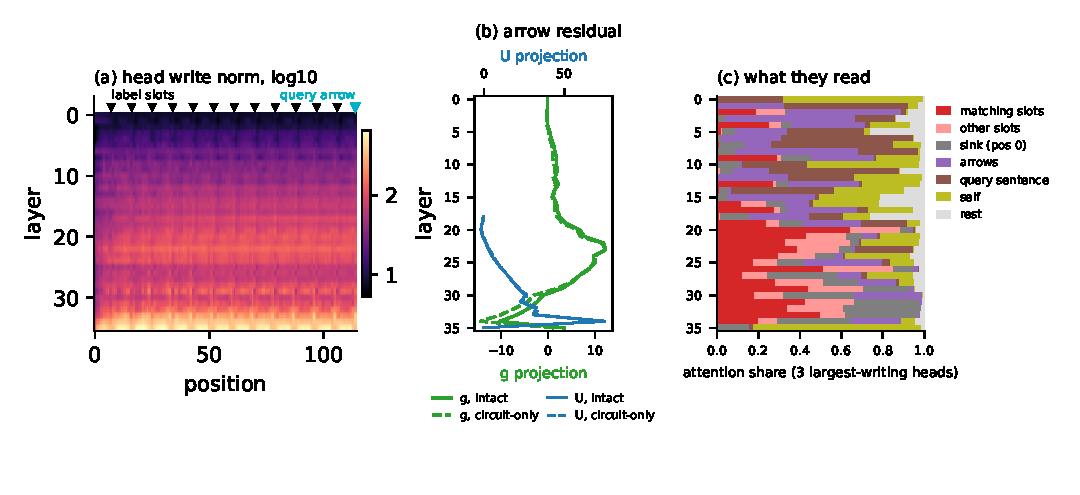
\includegraphics[width=\textwidth]{figures/fig19_trace.pdf}
\caption{Token observatory for one 12-shot prompt (symbol labels, answer \texttt{foo}) in Qwen3-4B. (a) Summed head write norm at every layer and position (log scale); white lines mark the label slots, cyan the query arrow. (b) At the query arrow, the residual's projection on the gate direction $g$ (green) and on the repeat-flag direction $U_l$ (blue) by layer, intact (solid) and with every unnamed head mean-ablated at the arrow (dashed). (c) Attention of the three heads that write most at the arrow in each layer, split by what they read.}
\label{fig:trace}
\end{figure}

\section{Completeness screen of layers 20--27}\label{app:complete}
Section~\ref{sec:accounting} located what the named set lacks to the unnamed heads of layers 20--27 at the query. To name them we mean-ablated each of the 256 heads in those layers alone at the query (reference: the head's mean output over the battery), 144 prompts per head, and measured the paired change in margin. The screen is a test of the named set as well as a search: the four largest single-head effects are named readers (23:26 $-0.11$, 22:10 $-0.11$, 22:13 $-0.10$, 24:22 $-0.09$ nats), and 11 of the 33 named heads in the band cost more than 0.02 against 17 of the 223 unnamed ones. Of the unnamed heads, 160 change the margin by less than 0.01 in either direction. Eight have an effect below $-0.03$ with a confidence interval excluding zero: four of them put 0.48--0.61 of their attention on the recurring-label slots and are readers that the top-20 ranking missed (24:23 $-0.06$, 22:22 $-0.05$, 22:23 $-0.04$, 24:13 $-0.04$); the other four attend almost nowhere on the slots (0.01--0.10) and their attention rows at the query say what they are: 20:5 and 23:25 put 0.79 and 0.59 of their mass on the query sentence's own tokens, so they are query heads of the kind already named (22:10, 23:26), writing the query's class code into the arrow; 27:12 and 20:17 put 0.55 and 0.34 on the demonstration arrows (and 0.29 / 0.10 on the sink), so they read the prompt-level state that the pooling stage writes at the arrows. Knocking the four together on a fresh draw costs $-0.25$ / $-0.12$ nats (rare / symbol) against $+0.03$ / $+0.03$ for layer-matched random quadruples. All eight screened heads are instances of parts the account already has. None is a new stage. A further seven unnamed heads have effects of $-0.015$ to $-0.03$ with intervals excluding zero.

The band's joint cost is larger than the sum of its parts' signed effects (layers 22--23: $-0.36$ / $-0.19$ nats jointly, against a signed sum of single-head effects of $-0.01$ / $-0.08$; negatives alone sum to $-0.32$). Heads whose removal helps on its own ($+0.28$ in that band) do not help once the others are gone, which is what a distributed population looks like and is the same shape as the gain-versus-information result of Section~\ref{sec:arrows}. Adding the screened heads to the named set (79 heads) and rerunning the band test with the reference matched on label pair (Section~\ref{sec:transfer}) shrinks it: removing every remaining unnamed head of layers 20--27 at the query costs $-0.10$ / $-0.07$ nats (rare / symbol; before the screen $-0.67$ / $-0.34$), and the unnamed heads of 28--35 help when removed ($+0.17$ / $+0.09$), so beyond our set the late heads are brakes on average. Circuit-only with the 79-head set keeps about 60\% of the margin on both label kinds: $-0.47$ / $-0.28$ under resample ablation (intact $+1.14$ / $+0.55$; random set $-0.98$ / $-0.65$, no heads $-0.95$ / $-0.69$), $-0.26$ / $-0.22$ with the mean reference. The rest is split between the unnamed heads of layers 0--19 at the query ($-0.29$ / $-0.16$ in the band test), the encoder that computes the query sentence's class code at the arrow and that this account takes as the circuit's input rather than as one of its parts, and a thin tail of layers 20--27. The natural-label screen of Section~\ref{sec:transfer} names that tail together with the late brakes (110 heads), and the final 189-head set is above intact on this battery too ($+1.26$ / $+0.89$ under resample, $+1.62$ / $+0.93$ with the mean reference; random $-0.98$ / $-0.64$), with layers 20--27 and 28--35 helping when their leftover heads go ($+0.99$ / $+0.40$, $+0.65$ / $+0.35$) and layers 0--19 costing $-0.17$ / $-0.07$. An earlier version of this test used the battery mean over both label pairs and a resample partner one row on, which in this battery is the same prompt under the other pair; it read $+0.49$ on symbol labels for the 79-head set, and that number was the partner's doing. The attention rows of all eight heads at the query are in the released data.

\paragraph{Layers 0--19.} The same screen over the 640 heads of layers 0--19 at the query (five containers, 144 prompts per head) finds no part. One head crosses $-0.03$ (8:23, $-0.037$); three more lie between $-0.02$ and $-0.03$ (19:24, 6:20, 6:15); the remaining 636 are within $\pm0.02$ of zero, and only two help when removed. The band knocks are small and shrink with depth: layers 0--3 $+0.00$ / $-0.01$, 4--7 $-0.09$ / $-0.05$, 8--11 $-0.05$ / $-0.02$, 12--15 $-0.02$ / $-0.02$, 16--19 $-0.11$ / $-0.06$ (rare / symbol; intervals for 0--3, 12--15 and the symbol value of 16--19 include zero). The 16--19 band holds the one early head that looks like a reader (19:11, 0.89 of its attention on the recurring slots, $-0.015$) and the second-largest early effect (19:24, $-0.029$, which attends to neither slots nor sink). Knocking the four largest early heads together (8:23, 6:20, 6:15, 7:31) on a fresh draw costs $-0.06$ / $-0.02$ against $0.00$ for random quadruples. Their attention rows say what little they do: 8:23 puts 0.97 of its mass on the demonstration arrows (an early reader of prompt-level state, the kind of input the pooling stage uses), 6:20 and 7:31 put 0.97 and 0.68 on the query sentence (early copies of the query's words into the arrow, upstream of the query heads), and 6:15 is mixed. We had predicted, before reading them, that the early heads that matter for rare labels would attend to the label slots and carry a label-type feature; they do not, so that hypothesis is dropped and the rare-label remainder stays unexplained at the level of parts. This is what the gain bound predicts for heads whose output-value map has little component along a late answer direction: the early layers contribute to the margin as substrate, a few hundredths of a nat per head, not as parts. Adding those four to the named set (91 heads) does not close the early band ($-0.35$ / $-0.18$ when every other layer 0--19 head is removed at the query, against $-0.38$ / $-0.16$ before), which is the point: the early contribution is the sum of six hundred effects of a few thousandths each, not a part one could name. With the 91-head set, circuit-only keeps 65\% of the rare-label margin ($-0.40$ from $+1.13$; random set $-0.75$, no heads $-0.72$) and on symbol labels is indistinguishable from intact under battery means ($-0.19$, interval includes zero) and above intact under resample ($+0.46$).

\section{Components or populations}\label{app:populations}
Of the links in Table~\ref{tab:replication}, the two query computers, the sixteen duplicate-token heads, the three value groups, SmolLM3's three order carriers and the four-demonstration label-prior neurons are small named sets; the writers, the 89 slot-reading readers, the roughly thirty gate-released heads and the 24 brakes are populations in which no single unit is necessary. The population links are forced by gain: a reader's class bias is 0.2--0.4 nats on a 0.5-nat per-slot spread, and no head's output writes more than 0.2 nats of answer logit, so a 1.3-nat class flip is a sum over at least seven heads and in practice over tens. Units move while the function stays (Section~\ref{sec:discussion}). The architecture-forced parts of the account, the null action and the within-regime read law, follow from the softmax and the causal mask and appear in every model we tested.
\end{document}
